
% Default to the notebook output style

    


% Inherit from the specified cell style.




    
\documentclass{article}

    
    
    \usepackage{graphicx} % Used to insert images
    \usepackage{adjustbox} % Used to constrain images to a maximum size 
    \usepackage{color} % Allow colors to be defined
    \usepackage{enumerate} % Needed for markdown enumerations to work
    \usepackage{geometry} % Used to adjust the document margins
    \usepackage{amsmath} % Equations
    \usepackage{amssymb} % Equations
    \usepackage{eurosym} % defines \euro
    \usepackage[mathletters]{ucs} % Extended unicode (utf-8) support
    \usepackage[utf8x]{inputenc} % Allow utf-8 characters in the tex document
    \usepackage{fancyvrb} % verbatim replacement that allows latex
    \usepackage{grffile} % extends the file name processing of package graphics 
                         % to support a larger range 
    % The hyperref package gives us a pdf with properly built
    % internal navigation ('pdf bookmarks' for the table of contents,
    % internal cross-reference links, web links for URLs, etc.)
    \usepackage{hyperref}
    \usepackage{longtable} % longtable support required by pandoc >1.10
    \usepackage{booktabs}  % table support for pandoc > 1.12.2
    \usepackage{mathpazo}
    \usepackage[spanish]{babel}

    \DeclareMathOperator{\adjunta}{adj}

    
    
    \definecolor{orange}{cmyk}{0,0.4,0.8,0.2}
    \definecolor{darkorange}{rgb}{.71,0.21,0.01}
    \definecolor{darkgreen}{rgb}{.12,.54,.11}
    \definecolor{myteal}{rgb}{.26, .44, .56}
    \definecolor{gray}{gray}{0.45}
    \definecolor{lightgray}{gray}{.95}
    \definecolor{mediumgray}{gray}{.8}
    \definecolor{inputbackground}{rgb}{.95, .95, .85}
    \definecolor{outputbackground}{rgb}{.95, .95, .95}
    \definecolor{traceback}{rgb}{1, .95, .95}
    % ansi colors
    \definecolor{red}{rgb}{.6,0,0}
    \definecolor{green}{rgb}{0,.65,0}
    \definecolor{brown}{rgb}{0.6,0.6,0}
    \definecolor{blue}{rgb}{0,.145,.698}
    \definecolor{purple}{rgb}{.698,.145,.698}
    \definecolor{cyan}{rgb}{0,.698,.698}
    \definecolor{lightgray}{gray}{0.5}
    
    % bright ansi colors
    \definecolor{darkgray}{gray}{0.25}
    \definecolor{lightred}{rgb}{1.0,0.39,0.28}
    \definecolor{lightgreen}{rgb}{0.48,0.99,0.0}
    \definecolor{lightblue}{rgb}{0.53,0.81,0.92}
    \definecolor{lightpurple}{rgb}{0.87,0.63,0.87}
    \definecolor{lightcyan}{rgb}{0.5,1.0,0.83}
    
    % commands and environments needed by pandoc snippets
    % extracted from the output of `pandoc -s`
    \DefineVerbatimEnvironment{Highlighting}{Verbatim}{commandchars=\\\{\}}
    % Add ',fontsize=\small' for more characters per line
    \newenvironment{Shaded}{}{}
    \newcommand{\KeywordTok}[1]{\textcolor[rgb]{0.00,0.44,0.13}{\textbf{{#1}}}}
    \newcommand{\DataTypeTok}[1]{\textcolor[rgb]{0.56,0.13,0.00}{{#1}}}
    \newcommand{\DecValTok}[1]{\textcolor[rgb]{0.25,0.63,0.44}{{#1}}}
    \newcommand{\BaseNTok}[1]{\textcolor[rgb]{0.25,0.63,0.44}{{#1}}}
    \newcommand{\FloatTok}[1]{\textcolor[rgb]{0.25,0.63,0.44}{{#1}}}
    \newcommand{\CharTok}[1]{\textcolor[rgb]{0.25,0.44,0.63}{{#1}}}
    \newcommand{\StringTok}[1]{\textcolor[rgb]{0.25,0.44,0.63}{{#1}}}
    \newcommand{\CommentTok}[1]{\textcolor[rgb]{0.38,0.63,0.69}{\textit{{#1}}}}
    \newcommand{\OtherTok}[1]{\textcolor[rgb]{0.00,0.44,0.13}{{#1}}}
    \newcommand{\AlertTok}[1]{\textcolor[rgb]{1.00,0.00,0.00}{\textbf{{#1}}}}
    \newcommand{\FunctionTok}[1]{\textcolor[rgb]{0.02,0.16,0.49}{{#1}}}
    \newcommand{\RegionMarkerTok}[1]{{#1}}
    \newcommand{\ErrorTok}[1]{\textcolor[rgb]{1.00,0.00,0.00}{\textbf{{#1}}}}
    \newcommand{\NormalTok}[1]{{#1}}
    
    % Define a nice break command that doesn't care if a line doesn't already
    % exist.
    \def\br{\hspace*{\fill} \\* }
    % Math Jax compatability definitions
    \def\gt{>}
    \def\lt{<}
    % Document parameters
    \title{Pendubot}
    
    
    

    % Pygments definitions
    
\makeatletter
\def\PY@reset{\let\PY@it=\relax \let\PY@bf=\relax%
    \let\PY@ul=\relax \let\PY@tc=\relax%
    \let\PY@bc=\relax \let\PY@ff=\relax}
\def\PY@tok#1{\csname PY@tok@#1\endcsname}
\def\PY@toks#1+{\ifx\relax#1\empty\else%
    \PY@tok{#1}\expandafter\PY@toks\fi}
\def\PY@do#1{\PY@bc{\PY@tc{\PY@ul{%
    \PY@it{\PY@bf{\PY@ff{#1}}}}}}}
\def\PY#1#2{\PY@reset\PY@toks#1+\relax+\PY@do{#2}}

\expandafter\def\csname PY@tok@s\endcsname{\def\PY@tc##1{\textcolor[rgb]{0.73,0.13,0.13}{##1}}}
\expandafter\def\csname PY@tok@s2\endcsname{\def\PY@tc##1{\textcolor[rgb]{0.73,0.13,0.13}{##1}}}
\expandafter\def\csname PY@tok@sc\endcsname{\def\PY@tc##1{\textcolor[rgb]{0.73,0.13,0.13}{##1}}}
\expandafter\def\csname PY@tok@k\endcsname{\let\PY@bf=\textbf\def\PY@tc##1{\textcolor[rgb]{0.00,0.50,0.00}{##1}}}
\expandafter\def\csname PY@tok@sb\endcsname{\def\PY@tc##1{\textcolor[rgb]{0.73,0.13,0.13}{##1}}}
\expandafter\def\csname PY@tok@gd\endcsname{\def\PY@tc##1{\textcolor[rgb]{0.63,0.00,0.00}{##1}}}
\expandafter\def\csname PY@tok@ss\endcsname{\def\PY@tc##1{\textcolor[rgb]{0.10,0.09,0.49}{##1}}}
\expandafter\def\csname PY@tok@ni\endcsname{\let\PY@bf=\textbf\def\PY@tc##1{\textcolor[rgb]{0.60,0.60,0.60}{##1}}}
\expandafter\def\csname PY@tok@mo\endcsname{\def\PY@tc##1{\textcolor[rgb]{0.40,0.40,0.40}{##1}}}
\expandafter\def\csname PY@tok@gr\endcsname{\def\PY@tc##1{\textcolor[rgb]{1.00,0.00,0.00}{##1}}}
\expandafter\def\csname PY@tok@err\endcsname{\def\PY@bc##1{\setlength{\fboxsep}{0pt}\fcolorbox[rgb]{1.00,0.00,0.00}{1,1,1}{\strut ##1}}}
\expandafter\def\csname PY@tok@ow\endcsname{\let\PY@bf=\textbf\def\PY@tc##1{\textcolor[rgb]{0.67,0.13,1.00}{##1}}}
\expandafter\def\csname PY@tok@nn\endcsname{\let\PY@bf=\textbf\def\PY@tc##1{\textcolor[rgb]{0.00,0.00,1.00}{##1}}}
\expandafter\def\csname PY@tok@kn\endcsname{\let\PY@bf=\textbf\def\PY@tc##1{\textcolor[rgb]{0.00,0.50,0.00}{##1}}}
\expandafter\def\csname PY@tok@vc\endcsname{\def\PY@tc##1{\textcolor[rgb]{0.10,0.09,0.49}{##1}}}
\expandafter\def\csname PY@tok@nv\endcsname{\def\PY@tc##1{\textcolor[rgb]{0.10,0.09,0.49}{##1}}}
\expandafter\def\csname PY@tok@kp\endcsname{\def\PY@tc##1{\textcolor[rgb]{0.00,0.50,0.00}{##1}}}
\expandafter\def\csname PY@tok@gi\endcsname{\def\PY@tc##1{\textcolor[rgb]{0.00,0.63,0.00}{##1}}}
\expandafter\def\csname PY@tok@cm\endcsname{\let\PY@it=\textit\def\PY@tc##1{\textcolor[rgb]{0.25,0.50,0.50}{##1}}}
\expandafter\def\csname PY@tok@c\endcsname{\let\PY@it=\textit\def\PY@tc##1{\textcolor[rgb]{0.25,0.50,0.50}{##1}}}
\expandafter\def\csname PY@tok@nb\endcsname{\def\PY@tc##1{\textcolor[rgb]{0.00,0.50,0.00}{##1}}}
\expandafter\def\csname PY@tok@kr\endcsname{\let\PY@bf=\textbf\def\PY@tc##1{\textcolor[rgb]{0.00,0.50,0.00}{##1}}}
\expandafter\def\csname PY@tok@sd\endcsname{\let\PY@it=\textit\def\PY@tc##1{\textcolor[rgb]{0.73,0.13,0.13}{##1}}}
\expandafter\def\csname PY@tok@ne\endcsname{\let\PY@bf=\textbf\def\PY@tc##1{\textcolor[rgb]{0.82,0.25,0.23}{##1}}}
\expandafter\def\csname PY@tok@s1\endcsname{\def\PY@tc##1{\textcolor[rgb]{0.73,0.13,0.13}{##1}}}
\expandafter\def\csname PY@tok@se\endcsname{\let\PY@bf=\textbf\def\PY@tc##1{\textcolor[rgb]{0.73,0.40,0.13}{##1}}}
\expandafter\def\csname PY@tok@gh\endcsname{\let\PY@bf=\textbf\def\PY@tc##1{\textcolor[rgb]{0.00,0.00,0.50}{##1}}}
\expandafter\def\csname PY@tok@kd\endcsname{\let\PY@bf=\textbf\def\PY@tc##1{\textcolor[rgb]{0.00,0.50,0.00}{##1}}}
\expandafter\def\csname PY@tok@c1\endcsname{\let\PY@it=\textit\def\PY@tc##1{\textcolor[rgb]{0.25,0.50,0.50}{##1}}}
\expandafter\def\csname PY@tok@si\endcsname{\let\PY@bf=\textbf\def\PY@tc##1{\textcolor[rgb]{0.73,0.40,0.53}{##1}}}
\expandafter\def\csname PY@tok@sx\endcsname{\def\PY@tc##1{\textcolor[rgb]{0.00,0.50,0.00}{##1}}}
\expandafter\def\csname PY@tok@cp\endcsname{\def\PY@tc##1{\textcolor[rgb]{0.74,0.48,0.00}{##1}}}
\expandafter\def\csname PY@tok@ge\endcsname{\let\PY@it=\textit}
\expandafter\def\csname PY@tok@bp\endcsname{\def\PY@tc##1{\textcolor[rgb]{0.00,0.50,0.00}{##1}}}
\expandafter\def\csname PY@tok@nf\endcsname{\def\PY@tc##1{\textcolor[rgb]{0.00,0.00,1.00}{##1}}}
\expandafter\def\csname PY@tok@nd\endcsname{\def\PY@tc##1{\textcolor[rgb]{0.67,0.13,1.00}{##1}}}
\expandafter\def\csname PY@tok@gt\endcsname{\def\PY@tc##1{\textcolor[rgb]{0.00,0.27,0.87}{##1}}}
\expandafter\def\csname PY@tok@no\endcsname{\def\PY@tc##1{\textcolor[rgb]{0.53,0.00,0.00}{##1}}}
\expandafter\def\csname PY@tok@w\endcsname{\def\PY@tc##1{\textcolor[rgb]{0.73,0.73,0.73}{##1}}}
\expandafter\def\csname PY@tok@mh\endcsname{\def\PY@tc##1{\textcolor[rgb]{0.40,0.40,0.40}{##1}}}
\expandafter\def\csname PY@tok@kc\endcsname{\let\PY@bf=\textbf\def\PY@tc##1{\textcolor[rgb]{0.00,0.50,0.00}{##1}}}
\expandafter\def\csname PY@tok@sr\endcsname{\def\PY@tc##1{\textcolor[rgb]{0.73,0.40,0.53}{##1}}}
\expandafter\def\csname PY@tok@gp\endcsname{\let\PY@bf=\textbf\def\PY@tc##1{\textcolor[rgb]{0.00,0.00,0.50}{##1}}}
\expandafter\def\csname PY@tok@nc\endcsname{\let\PY@bf=\textbf\def\PY@tc##1{\textcolor[rgb]{0.00,0.00,1.00}{##1}}}
\expandafter\def\csname PY@tok@vi\endcsname{\def\PY@tc##1{\textcolor[rgb]{0.10,0.09,0.49}{##1}}}
\expandafter\def\csname PY@tok@kt\endcsname{\def\PY@tc##1{\textcolor[rgb]{0.69,0.00,0.25}{##1}}}
\expandafter\def\csname PY@tok@sh\endcsname{\def\PY@tc##1{\textcolor[rgb]{0.73,0.13,0.13}{##1}}}
\expandafter\def\csname PY@tok@nt\endcsname{\let\PY@bf=\textbf\def\PY@tc##1{\textcolor[rgb]{0.00,0.50,0.00}{##1}}}
\expandafter\def\csname PY@tok@m\endcsname{\def\PY@tc##1{\textcolor[rgb]{0.40,0.40,0.40}{##1}}}
\expandafter\def\csname PY@tok@il\endcsname{\def\PY@tc##1{\textcolor[rgb]{0.40,0.40,0.40}{##1}}}
\expandafter\def\csname PY@tok@gu\endcsname{\let\PY@bf=\textbf\def\PY@tc##1{\textcolor[rgb]{0.50,0.00,0.50}{##1}}}
\expandafter\def\csname PY@tok@mi\endcsname{\def\PY@tc##1{\textcolor[rgb]{0.40,0.40,0.40}{##1}}}
\expandafter\def\csname PY@tok@cs\endcsname{\let\PY@it=\textit\def\PY@tc##1{\textcolor[rgb]{0.25,0.50,0.50}{##1}}}
\expandafter\def\csname PY@tok@go\endcsname{\def\PY@tc##1{\textcolor[rgb]{0.53,0.53,0.53}{##1}}}
\expandafter\def\csname PY@tok@mb\endcsname{\def\PY@tc##1{\textcolor[rgb]{0.40,0.40,0.40}{##1}}}
\expandafter\def\csname PY@tok@o\endcsname{\def\PY@tc##1{\textcolor[rgb]{0.40,0.40,0.40}{##1}}}
\expandafter\def\csname PY@tok@nl\endcsname{\def\PY@tc##1{\textcolor[rgb]{0.63,0.63,0.00}{##1}}}
\expandafter\def\csname PY@tok@na\endcsname{\def\PY@tc##1{\textcolor[rgb]{0.49,0.56,0.16}{##1}}}
\expandafter\def\csname PY@tok@mf\endcsname{\def\PY@tc##1{\textcolor[rgb]{0.40,0.40,0.40}{##1}}}
\expandafter\def\csname PY@tok@vg\endcsname{\def\PY@tc##1{\textcolor[rgb]{0.10,0.09,0.49}{##1}}}
\expandafter\def\csname PY@tok@gs\endcsname{\let\PY@bf=\textbf}

\def\PYZbs{\char`\\}
\def\PYZus{\char`\_}
\def\PYZob{\char`\{}
\def\PYZcb{\char`\}}
\def\PYZca{\char`\^}
\def\PYZam{\char`\&}
\def\PYZlt{\char`\<}
\def\PYZgt{\char`\>}
\def\PYZsh{\char`\#}
\def\PYZpc{\char`\%}
\def\PYZdl{\char`\$}
\def\PYZhy{\char`\-}
\def\PYZsq{\char`\'}
\def\PYZdq{\char`\"}
\def\PYZti{\char`\~}
% for compatibility with earlier versions
\def\PYZat{@}
\def\PYZlb{[}
\def\PYZrb{]}
\makeatother


    % Exact colors from NB
    \definecolor{incolor}{rgb}{0.0, 0.0, 0.5}
    \definecolor{outcolor}{rgb}{0.545, 0.0, 0.0}



    
    % Prevent overflowing lines due to hard-to-break entities
    \sloppy 
    % Setup hyperref package
    \hypersetup{
      breaklinks=true,  % so long urls are correctly broken across lines
      colorlinks=true,
      urlcolor=blue,
      linkcolor=darkorange,
      citecolor=darkgreen,
      }
    % Slightly bigger margins than the latex defaults
    
    \geometry{verbose,tmargin=1cm,bmargin=1.5cm,lmargin=1cm,rmargin=1cm}
    
    \author{Roberto Cadena Vega}
    \date{24 de abril de 2015}

    \begin{document}
    
    
    \maketitle
    
    \section*{Examen Final}\label{examen-final}

    \subsection*{Modelado de pendubot}\label{modelado-de-pendubot}

    \begin{figure*}[htbp]
\centering
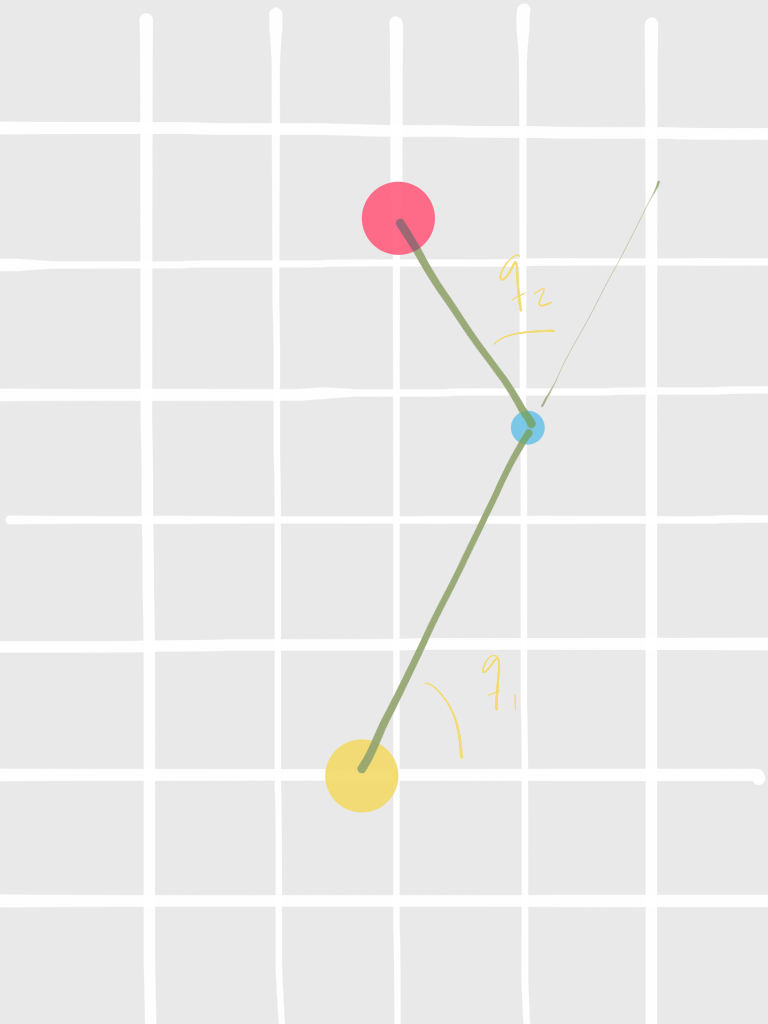
\includegraphics[width=0.3\linewidth]{./imagenes/doblependulo.PNG}
\end{figure*}

    \subsubsection*{Variables de estado, posiciones y
velocidades}\label{variables-de-estado-posiciones-y-velocidades}

    \[
q = 
\begin{pmatrix}
q_1 \\
q_2
\end{pmatrix} \implies
\dot{q} =
\begin{pmatrix}
\dot{q}_1 \\
\dot{q}_2
\end{pmatrix}
\]

Las posiciones de las juntas estan dadas por:

\[
\begin{align}
\begin{pmatrix}
x_1 & y_1
\end{pmatrix} &= 
\begin{pmatrix}
l_1 \cos{(q_1)} & l_1 \sin{(q_1)}
\end{pmatrix} \\
\begin{pmatrix}
x_2 & y_2
\end{pmatrix} &= 
\begin{pmatrix}
l_1 \cos{(q_1)} + l_2 \cos{(q_1 + q_2)} & l_1 \sin{(q_1)} + l_2 \sin{(q_1 + q_2)}
\end{pmatrix}
\end{align}
\]

y por lo tanto, las velocidades estarán dadas por:

\[
\begin{align}
\begin{pmatrix}
\dot{x}_1 & \dot{y}_1
\end{pmatrix} &= 
\begin{pmatrix}
-l_1 \sin{(q_1)} \dot{q}_1 & l_1 \cos{(q_1)} \dot{q}_1
\end{pmatrix} \\
\begin{pmatrix}
\dot{x}_2 & \dot{y}_2
\end{pmatrix} &= 
\begin{pmatrix}
-l_1 \sin{(q_1)} \dot{q}_1 - l_2 \sin{(q_1 + q_2)} (\dot{q}_1 + \dot{q}_2) & l_1 \cos{(q_1)} \dot{q}_1 + l_2 \cos{(q_1 + q_2)} (\dot{q}_1 + \dot{q}_2)
\end{pmatrix}
\end{align}
\]

    \subsubsection*{Energía cinética}\label{energuxeda-cinuxe9tica}

    Considerando que la velocidad \(v_i\) es la norma de estas componentes,
\(v_i = \sqrt{\dot{x}_i^2 + \dot{y}_i^2}\), la energía cinética del
sistema esta dada dada por:

\[
\begin{align}
K &= K_1 + K_2 \\
&= \frac{1}{2} m_1 v_1^2 + \frac{1}{2} m_2 v_2^2
\end{align}
\]

con \(v_1^2\) dada por:

\[
\begin{align}
v_1^2 &= \dot{x}_1^2 + \dot{y}_1^2 \\
&= l_1^2 \sin^2{(q_1)} \dot{q}_1^2 + l_1^2 \cos^2{(q_1)} \dot{q}_1^2 \\
&= l_1^2 \dot{q}_1^2
\end{align}
\]

y \(v_2^2\):

\[
\begin{align}
v_2^2 &= \dot{x}_2^2 + \dot{y}_2^2 \\
&= \left( -l_1 \sin{(q_1)} \dot{q}_1 - l_2 \sin{(q_1 + q_2)} (\dot{q}_1 + \dot{q}_2) \right)^2 + \left( l_1 \cos{(q_1)} \dot{q}_1 + l_2 \cos{(q_1 + q_2)} (\dot{q}_1 + \dot{q}_2) \right)^2 \\
&= l_1^2 \dot{q}_1^2 + l_2^2 (\dot{q}_1 + \dot{q}_2)^2 + 2\left[ l_1 \sin{(q_1)} \dot{q}_1 \cdot l_2 \sin{(q_1 + q_2)} (\dot{q}_1 + \dot{q}_2)
+ l_1 \cos{(q_1)} \dot{q}_1 \cdot l_2 \cos{(q_1 + q_2)} (\dot{q}_1 + \dot{q}_2) \right] \\
&= l_1^2 \dot{q}_1^2 + l_2^2 (\dot{q}_1 + \dot{q}_2)^2 + 2 l_1 l_2 \left[ \sin{(q_1)} \sin{(q_1 + q_2)} + \cos{(q_1)} \cos{(q_1 + q_2)} \right] \dot{q}_1 (\dot{q}_1 + \dot{q}_2) \\
&= l_1^2 \dot{q}_1^2 + l_2^2 (\dot{q}_1 + \dot{q}_2)^2 + 2 l_1 l_2 \cos{(q_2)} \dot{q}_1 (\dot{q}_1 + \dot{q}_2)
\end{align}
\]

por lo que las energías cinéticas de cada junta quedan:

\[
\begin{align}
K_1 &= \frac{1}{2} m_1 v_1^2 = \frac{1}{2} m_1 l_1^2 \dot{q}_1^2 \\
K_2 &= \frac{1}{2} m_2 v_2^2 = \frac{1}{2} m_2 \left[ l_1^2 \dot{q}_1^2 + l_2^2 (\dot{q}_1 + \dot{q}_2)^2 + 2 l_1 l_2 \cos{(q_2)} \dot{q}_1 (\dot{q}_1 + \dot{q}_2) \right] \\
&= \frac{1}{2} m_2 \left[ l_1^2 \dot{q}_1^2 + l_2^2 \dot{q}_1^2 + l_2^2 \dot{q}_2^2 + 2 l_2^2 \dot{q}_1 \dot{q}_2 + 2 l_1 l_2 \cos{(q_2)} \dot{q}_1^2 + 2 l_1 l_2 \cos{(q_2)} \dot{q}_1 \dot{q}_2 \right] \\
&= \frac{1}{2} m_2 \left[ \left( l_1^2 + l_2^2 + 2 l_1 l_2 \cos{(q_2)} \right) \dot{q}_1^2 + l_2^2 \dot{q}_2^2 + 2 \left( l_2^2 + l_1 l_2 \cos{(q_2)} \right) \dot{q}_1 \dot{q}_2 \right]
\end{align}
\]

por lo que la energía cinética total, será:

\[
\begin{align}
K &= K_1 + K_2 \\
&= \frac{1}{2} m_1 l_1^2 \dot{q}_1^2 + \frac{1}{2} m_2 \left[ \left( l_1^2 + l_2^2 + 2 l_1 l_2 \cos{(q_2)} \right) \dot{q}_1^2 + l_2^2 \dot{q}_2^2 + 2 \left( l_2^2 + l_1 l_2 \cos{(q_2)} \right) \dot{q}_1 \dot{q}_2 \right] \\
&= \frac{1}{2} \left\{ m_1 l_1^2 \dot{q}_1^2 + m_2 \left[ \left( l_1^2 + l_2^2 + 2 l_1 l_2 \cos{(q_2)} \right) \dot{q}_1^2 + l_2^2 \dot{q}_2^2 + 2 \left( l_2^2 + l_1 l_2 \cos{(q_2)} \right) \dot{q}_1 \dot{q}_2 \right] \right\} \\
&= \frac{1}{2} \left\{ \left[ m_1 l_1^2 + m_2 \left( l_1^2 + l_2^2 + 2 l_1 l_2 \cos{(q_2)} \right) \right] \dot{q}_1^2 + m_2 l_2^2 \dot{q}_2^2 + 2 m_2 \left( l_2^2 + l_1 l_2 \cos{(q_2)} \right) \dot{q}_1 \dot{q}_2\right\} \\
&= \frac{1}{2} \left\{ \left[ (m_1 + m_2) l_1^2 + m_2 l_2^2 + 2 m_2 l_1 l_2 \cos{(q_2)} \right] \dot{q}_1^2 + m_2 l_2^2 \dot{q}_2^2 + 2 m_2 \left( l_2^2 + l_1 l_2 \cos{(q_2)} \right) \dot{q}_1 \dot{q}_2\right\} \\
\end{align}
\]

La cual, al ver las relaciones con las variables de posición
generalizadas del pendulo, podemos escribir como:

\[
K = \frac{1}{2} \dot{q}^T M(q) \dot{q}
\]

en donde la matriz de inercia \(M(q)\) queda de la forma:

\[
M(q) =
\begin{pmatrix}
(m_1 + m_2) l_1^2 + m_2 l_2^2 + 2 m_2 l_1 l_2 \cos{(q_2)} & m_2 l_2^2 + m_2 l_1 l_2 \cos{(q_2)} \\
m_2 l_2^2 + m_2 l_1 l_2 \cos{(q_2)} & m_2 l_2^2
\end{pmatrix}
\]

en donde podemos introducir las constantes \(\mu_i\) para simplificar la
notación:

\[
\begin{align}
\mu_1 &= (m_1 + m_2) l_1^2 \\
\mu_2 &= m_2 l_2^2 \\
\mu_3 &= m_2 l_1 l_2
\end{align}
\]

con lo que la expresión para la energía cinética queda:

\[
K = \frac{1}{2} \dot{q}^T
\begin{pmatrix}
\mu_1 + \mu_2 + 2\mu_3 \cos{(q_2)} & \mu_2 + \mu_3 \cos{(q_2)} \\
\mu_2 + \mu_3 \cos{(q_2)} & \mu_2
\end{pmatrix} \dot{q}
\]

    \subsubsection*{Energía potencial}\label{energuxeda-potencial}

    La energía potencial del sistema esta dada por:

\[
\begin{align}
U &= U_1 + U_2 \\
&= m_1 g h_1 + m_2 g h_2 \\
&= m_1 g y_1 + m_2 g y_2 \\
&= m_1 g l_1 \sin{(q_1)} + m_2 g \left[ l_1 \sin{(q_1)} + l_2 \sin{(q_1 + q_2)} \right] \\
&= \left( m_1 + m_2 \right) g l_1 \sin{(q_1)} + m_2 g l_2 \sin{(q_1 + q_2)} \\
&= g \left[ \left( m_1 + m_2 \right) l_1 \sin{(q_1)} + m_2 l_2 \sin{(q_1 + q_2)} \right] \\
\end{align}
\]

    \subsubsection*{Lagrangiano}\label{lagrangiano}

    El Lagrangiano del sistema, esta dado por la expresión:

\[
L = K - U
\]

por lo que solo queda sumar las dos expresiones y obtener las
condiciones de optimalidad para la energía del sistema por medio de la
ecuación de Euler-Lagrange

    \subsubsection*{Euler-Lagrange}\label{euler-lagrange}

    \[
\frac{d}{dt} \left( \frac{\partial L}{\partial \dot{q}} \right) - \frac{\partial L}{\partial q} = 0
\]

Si empezamos derivando con respecto a \(\dot{q}\), tendremos:

\[
\frac{\partial L}{\partial \dot{q}} = \frac{\partial K}{\partial \dot{q}} - \frac{\partial U}{\partial \dot{q}}
\]

y obteniendo cada uno de estos tenemos que:

\[
\begin{align}
\frac{\partial K}{\partial \dot{q}} &= K_{\dot{q}} = \frac{\partial}{\partial \dot{q}} \left\{ \frac{1}{2} \dot{q}^T M(q) \dot{q} \right\} = M(q) \dot{q} \\
\frac{\partial U}{\partial \dot{q}} &= U_{\dot{q}} = 0
\end{align}
\]

y la derivada con respecto al tiempo de estos terminos será:

\[
\begin{align}
\frac{d K_{\dot{q}}}{dt} &= M(q) \ddot{q} + \dot{M}(q, \dot{q}) \dot{q} \\
\frac{d U_{\dot{q}}}{dt} &= 0
\end{align}
\]

en donde:

\[
\begin{align}
\dot{M}(q, \dot{q}) &= \frac{d}{dt}
\begin{pmatrix}
\mu_1 + \mu_2 + 2\mu_3 \cos{(q_2)} & \mu_2 + \mu_3 \cos{(q_2)} \\
\mu_2 + \mu_3 \cos{(q_2)} & \mu_2
\end{pmatrix} \\
&=
\begin{pmatrix}
-2 \mu_3 \sin{(q_2)} \dot{q}_2 & -\mu_3 \sin{(q_2)} \dot{q}_2 \\
-\mu_3 \sin{(q_2)} \dot{q}_2 & 0
\end{pmatrix} \\
&= -\mu_3 \sin{(q_2)}
\begin{pmatrix}
2 \dot{q}_2 & \dot{q}_2 \\
\dot{q}_2 & 0
\end{pmatrix}
\end{align}
\]

Ahora, derivando con respecto a \(q\), tenemos:

\[
\frac{\partial L}{\partial q} = \frac{\partial K}{\partial q} - \frac{\partial U}{\partial q}
\]

en donde:

\[
\begin{align}
\frac{\partial K}{\partial q} = K_{q} &=
\begin{pmatrix}
\frac{\partial K}{\partial q_1} \\
\frac{\partial K}{\partial q_2}
\end{pmatrix} \\
&= \frac{1}{2}
\begin{pmatrix}
\frac{\partial}{\partial q_1} \left\{ \left[ (m_1 + m_2) l_1^2 + m_2 l_2^2 + 2 m_2 l_1 l_2 \cos{(q_2)} \right] \dot{q}_1^2 + m_2 l_2^2 \dot{q}_2^2 + 2 m_2 \left( l_2^2 + l_1 l_2 \cos{(q_2)} \right) \dot{q}_1 \dot{q}_2 \right\} \\
\frac{\partial}{\partial q_2} \left\{ \left[ (m_1 + m_2) l_1^2 + m_2 l_2^2 + 2 m_2 l_1 l_2 \cos{(q_2)} \right] \dot{q}_1^2 + m_2 l_2^2 \dot{q}_2^2 + 2 m_2 \left( l_2^2 + l_1 l_2 \cos{(q_2)} \right) \dot{q}_1 \dot{q}_2 \right\} \\
\end{pmatrix} \\
&= \frac{1}{2}
\begin{pmatrix}
0 \\
-2 m_2 l_1 l_2 \sin{(q_2)} \dot{q}_1^2 - 2 m_2 l_1 l_2 \sin{(q_2)} \dot{q}_1 \dot{q}_2 \\
\end{pmatrix} \\
&= - \mu_3 \sin{(q_2)}
\begin{pmatrix}
0 \\
\dot{q}_1^2 + \dot{q}_1 \dot{q}_2 \\
\end{pmatrix} = -\mu_3 \sin{(q_2)}
\begin{pmatrix}
\dot{q}_2 & -\dot{q}_1 \\
\dot{q}_1 + \dot{q}_2 & 0
\end{pmatrix} \dot{q}
\end{align}
\]

y para la energía potencial:

\[
\begin{align}
\frac{\partial U}{\partial q} = U_q &=
\begin{pmatrix}
\frac{\partial U}{\partial q_1} \\
\frac{\partial U}{\partial q_2}
\end{pmatrix} \\
&= g
\begin{pmatrix}
\frac{\partial}{\partial q_1} \left[ \left( m_1 + m_2 \right) l_1 \sin{(q_1)} + m_2 l_2 \sin{(q_1 + q_2)} \right] \\
\frac{\partial}{\partial q_2} \left[ \left( m_1 + m_2 \right) l_1 \sin{(q_1)} + m_2 l_2 \sin{(q_1 + q_2)} \right]
\end{pmatrix} \\
&= g
\begin{pmatrix}
\left( m_1 + m_2 \right) l_1 \cos{(q_1)} + m_2 l_2 \cos{(q_1 + q_2)} \\
m_2 l_2 \cos{(q_1 + q_2)}
\end{pmatrix}
\end{align}
\]

o bien:

\[
U_q = g
\begin{pmatrix}
\mu_4 \cos{(q_1)} + \mu_5 \cos{(q_1 + q_2)} \\
\mu_5 \cos{(q_1 + q_2)}
\end{pmatrix}
\]

con \(\mu_4 = \left( m_1 + m_2 \right) l_1\) y \(\mu_5 = m_2 l_2\), por
lo que la ecuación de Euler-Lagrange queda:

\[
\begin{align}
\frac{d}{dt} \left( \frac{\partial L}{\partial \dot{q}} \right) &- \frac{\partial L}{\partial q} = 0 \\
\frac{d K_{\dot{q}}}{dt} &- \left( K_q - U_q \right) = 0 \\
M(q) \ddot{q} + \dot{M}(q, \dot{q}) \dot{q} &- K_q + U_q = 0
\end{align}
\]

en donde recordando que \(K_q\) tiene la forma
\(F(q, \dot{q}) \dot{q}\), podemos juntar esta matriz con
\(\dot{M}(q, \dot{q})\) y obtener una expresión de la forma:

\[
M(q) \ddot{q} + C(q, \dot{q}) \dot{q} + U_q = 0
\]

en donde:

\[
\begin{align}
M(q) &=
\begin{pmatrix}
\mu_1 + \mu_2 + 2\mu_3 \cos{(q_2)} & \mu_2 + \mu_3 \cos{(q_2)} \\
\mu_2 + \mu_3 \cos{(q_2)} & \mu_2
\end{pmatrix} \\
C(q, \dot{q}) &= \dot{M}(q, \dot{q}) - F(q, \dot{q}) =
-\mu_3 \sin{(q_2)}
\begin{pmatrix}
\dot{q}_2 & \dot{q}_1 + \dot{q}_2 \\
-\dot{q}_1 & 0
\end{pmatrix} \\
U_q &= g
\begin{pmatrix}
\mu_4 \cos{(q_1)} + \mu_5 \cos{(q_1 + q_2)} \\
\mu_5 \cos{(q_1 + q_2)}
\end{pmatrix}
\end{align}
\]

con

\[
\begin{align}
\mu_1 &= (m_1 + m_2) l_1^2 \\
\mu_2 &= m_2 l_2^2 \\
\mu_3 &= m_2 l_1 l_2 \\
\mu_4 &= \left( m_1 + m_2 \right) l_1 \\
\mu_5 &= m_2 l_2
\end{align}
\]

sin embargo este modelo no considera las señales de control, por lo que
procederemos a analizar el sistema.

    \subsubsection*{Señales de control}\label{seuxf1ales-de-control}

    Nuestra señal de control escalar se deberá enlazar al actuador del
pendubot, el cual esta asociado al primer grado de libertad \(q_1\), por
lo que finalmente tenemos la ecuación:

\[
M(q) \ddot{q} + C(q, \dot{q}) \dot{q} + U_q = G u
\]

con:

\[
G =
\begin{pmatrix}
1 \\
0
\end{pmatrix}
\]

    \begin{Verbatim}[commandchars=\\\{\}]
{\color{incolor}In [{\color{incolor}2}]:} \PY{k}{def} \PY{n+nf}{f}\PY{p}{(}\PY{n}{estado}\PY{p}{,} \PY{n}{tiempo}\PY{p}{,} \PY{n}{K}\PY{p}{)}\PY{p}{:}
            \PY{l+s+sd}{\PYZsq{}\PYZsq{}\PYZsq{}Modelo matematico pendubot}
        \PY{l+s+sd}{    Esta función f es tal que ẋ = f(x, t), es decir, dado el estado del sistema \PYZdq{}x\PYZdq{}}
        \PY{l+s+sd}{    y el tiempo \PYZdq{}t\PYZdq{}, devuelve la derivada en el tiempo \PYZdq{}t\PYZdq{}. Para el caso del pendubot,}
        \PY{l+s+sd}{    es invariante en el tiempo, por lo que es equivalente a ẋ = f(x).}
        
        \PY{l+s+sd}{    Ejemplo}
        \PY{l+s+sd}{    \PYZhy{}\PYZhy{}\PYZhy{}\PYZhy{}\PYZhy{}\PYZhy{}\PYZhy{}}
        \PY{l+s+sd}{    \PYZgt{}\PYZgt{}\PYZgt{} x = [τ/4, 0.1, 0, 0]}
        \PY{l+s+sd}{    \PYZgt{}\PYZgt{}\PYZgt{} t = 0}
        \PY{l+s+sd}{    \PYZgt{}\PYZgt{}\PYZgt{} f(x, t)}
        \PY{l+s+sd}{    array([  0.        ,   0.        ,  \PYZhy{}4.73091048,  17.41001448])}
        \PY{l+s+sd}{    \PYZsq{}\PYZsq{}\PYZsq{}}
            
            \PY{k+kn}{from} \PY{n+nn}{numpy} \PY{k}{import} \PY{n}{matrix}\PY{p}{,} \PY{n}{zeros}\PY{p}{,} \PY{n}{cos}\PY{p}{,} \PY{n}{sin}\PY{p}{,} \PY{n}{pi}
            
            \PY{c}{\PYZsh{} Constantes fisicas del sistema}
            \PY{n}{m1} \PY{o}{=} \PY{l+m+mf}{0.2} \PY{c}{\PYZsh{} kg}
            \PY{n}{m2} \PY{o}{=} \PY{l+m+mf}{0.6} \PY{c}{\PYZsh{} kg}
            \PY{n}{l1} \PY{o}{=} \PY{l+m+mf}{0.6} \PY{c}{\PYZsh{} m}
            \PY{n}{l2} \PY{o}{=} \PY{l+m+mf}{0.3} \PY{c}{\PYZsh{} m}
            \PY{n}{g} \PY{o}{=} \PY{l+m+mf}{9.81} \PY{c}{\PYZsh{} m/s\PYZca{}2}
            \PY{n}{τ} \PY{o}{=} \PY{l+m+mi}{2}\PY{o}{*}\PY{n}{pi}
            
            \PY{c}{\PYZsh{} Variables auxiliares del sistema}
            \PY{n}{μ1} \PY{o}{=} \PY{p}{(}\PY{n}{m1} \PY{o}{+} \PY{n}{m2}\PY{p}{)}\PY{o}{*}\PY{n}{l1}\PY{o}{*}\PY{o}{*}\PY{l+m+mi}{2}
            \PY{n}{μ2} \PY{o}{=} \PY{n}{m2}\PY{o}{*}\PY{n}{l2}\PY{o}{*}\PY{o}{*}\PY{l+m+mi}{2}
            \PY{n}{μ3} \PY{o}{=} \PY{n}{m2}\PY{o}{*}\PY{n}{l1}\PY{o}{*}\PY{n}{l2}
            \PY{n}{μ4} \PY{o}{=} \PY{p}{(}\PY{n}{m1} \PY{o}{+} \PY{n}{m2}\PY{p}{)}\PY{o}{*}\PY{n}{l1}
            \PY{n}{μ5} \PY{o}{=} \PY{n}{m2}\PY{o}{*}\PY{n}{l2}
            
            \PY{c}{\PYZsh{} Estado agregado}
            \PY{n}{q1}\PY{p}{,} \PY{n}{q2}\PY{p}{,} \PY{n}{q̇1}\PY{p}{,} \PY{n}{q̇2} \PY{o}{=} \PY{n}{estado}
            
            \PY{c}{\PYZsh{} Estado del sistema y derivada}
            \PY{n}{q} \PY{o}{=} \PY{n}{matrix}\PY{p}{(}\PY{p}{[}\PY{p}{[}\PY{n}{q1}\PY{p}{]}\PY{p}{,} \PY{p}{[}\PY{n}{q2}\PY{p}{]}\PY{p}{]}\PY{p}{)}
            \PY{n}{q̇} \PY{o}{=} \PY{n}{matrix}\PY{p}{(}\PY{p}{[}\PY{p}{[}\PY{n}{q̇1}\PY{p}{]}\PY{p}{,} \PY{p}{[}\PY{n}{q̇2}\PY{p}{]}\PY{p}{]}\PY{p}{)}
            
            \PY{c}{\PYZsh{} Matrix de inercia generalizada}
            \PY{n}{M} \PY{o}{=} \PY{n}{matrix}\PY{p}{(}\PY{p}{[}\PY{p}{[}\PY{n}{μ1} \PY{o}{+} \PY{n}{μ2} \PY{o}{+} \PY{l+m+mi}{2}\PY{o}{*}\PY{n}{μ3}\PY{o}{*}\PY{n}{cos}\PY{p}{(}\PY{n}{q2}\PY{p}{)}\PY{p}{,} \PY{n}{μ2} \PY{o}{+} \PY{n}{μ3}\PY{o}{*}\PY{n}{cos}\PY{p}{(}\PY{n}{q2}\PY{p}{)}\PY{p}{]}\PY{p}{,}
                        \PY{p}{[}\PY{n}{μ2} \PY{o}{+} \PY{n}{μ3}\PY{o}{*}\PY{n}{cos}\PY{p}{(}\PY{n}{q2}\PY{p}{)}\PY{p}{,} \PY{n}{μ2}\PY{p}{]}\PY{p}{]}\PY{p}{)}
            
            \PY{c}{\PYZsh{} Matriz de Coriolis}
            \PY{n}{C} \PY{o}{=} \PY{o}{\PYZhy{}}\PY{n}{μ3}\PY{o}{*}\PY{n}{sin}\PY{p}{(}\PY{n}{q2}\PY{p}{)}\PY{o}{*}\PY{n}{matrix}\PY{p}{(}\PY{p}{[}\PY{p}{[} \PY{n}{q̇2}\PY{p}{,} \PY{n}{q̇1} \PY{o}{+} \PY{n}{q̇2}\PY{p}{]}\PY{p}{,}
                                     \PY{p}{[}\PY{o}{\PYZhy{}}\PY{n}{q̇1}\PY{p}{,} \PY{l+m+mi}{0}\PY{p}{]}\PY{p}{]}\PY{p}{)}
            
            \PY{c}{\PYZsh{} Vector de gravedad}
            \PY{n}{U} \PY{o}{=} \PY{n}{g}\PY{o}{*}\PY{n}{matrix}\PY{p}{(}\PY{p}{[}\PY{p}{[}\PY{n}{μ4}\PY{o}{*}\PY{n}{cos}\PY{p}{(}\PY{n}{q1}\PY{p}{)} \PY{o}{+} \PY{n}{μ5}\PY{o}{*}\PY{n}{cos}\PY{p}{(}\PY{n}{q1} \PY{o}{+} \PY{n}{q2}\PY{p}{)}\PY{p}{]}\PY{p}{,}
                          \PY{p}{[}\PY{n}{μ5}\PY{o}{*}\PY{n}{cos}\PY{p}{(}\PY{n}{q1} \PY{o}{+} \PY{n}{q2}\PY{p}{)}\PY{p}{]}\PY{p}{]}\PY{p}{)}
            
            \PY{c}{\PYZsh{} Vector de señales de control}
            \PY{n}{G} \PY{o}{=} \PY{n}{matrix}\PY{p}{(}\PY{p}{[}\PY{p}{[}\PY{l+m+mi}{1}\PY{p}{]}\PY{p}{,} \PY{p}{[}\PY{l+m+mi}{0}\PY{p}{]}\PY{p}{]}\PY{p}{)}
            
            \PY{n}{ξ} \PY{o}{=} \PY{n}{matrix}\PY{p}{(}\PY{n}{estado}\PY{p}{)}\PY{o}{.}\PY{n}{T} \PY{o}{\PYZhy{}} \PY{n}{matrix}\PY{p}{(}\PY{p}{[}\PY{p}{[}\PY{n}{τ}\PY{o}{/}\PY{l+m+mi}{4}\PY{p}{]}\PY{p}{,} \PY{p}{[}\PY{l+m+mi}{0}\PY{p}{]}\PY{p}{,} \PY{p}{[}\PY{l+m+mi}{0}\PY{p}{]}\PY{p}{,} \PY{p}{[}\PY{l+m+mi}{0}\PY{p}{]}\PY{p}{]}\PY{p}{)}
            
            \PY{c}{\PYZsh{} Ley de control}
            \PY{n}{u} \PY{o}{=} \PY{o}{\PYZhy{}}\PY{p}{(}\PY{n}{matrix}\PY{p}{(}\PY{n}{K}\PY{p}{)}\PY{o}{*}\PY{n}{ξ}\PY{p}{)}\PY{o}{.}\PY{n}{tolist}\PY{p}{(}\PY{p}{)}\PY{p}{[}\PY{l+m+mi}{0}\PY{p}{]}\PY{p}{[}\PY{l+m+mi}{0}\PY{p}{]}
            
            \PY{c}{\PYZsh{} Aceleracion del sistema}
            \PY{n}{q̈} \PY{o}{=} \PY{n}{M}\PY{o}{.}\PY{n}{I}\PY{o}{*}\PY{p}{(}\PY{n}{G}\PY{o}{*}\PY{n}{u} \PY{o}{\PYZhy{}} \PY{n}{C}\PY{o}{*}\PY{n}{q̇} \PY{o}{\PYZhy{}} \PY{n}{U}\PY{p}{)}
            
            \PY{c}{\PYZsh{} Incializamos la derivada del estado agregado}
            \PY{n}{ẏ} \PY{o}{=} \PY{n}{zeros}\PY{p}{(}\PY{l+m+mi}{4}\PY{p}{)}
            
            \PY{c}{\PYZsh{} Se asignan los valores a la derivada del estado agregado}
            \PY{n}{ẏ}\PY{p}{[}\PY{l+m+mi}{0}\PY{p}{]} \PY{o}{=} \PY{n}{q̇1}
            \PY{n}{ẏ}\PY{p}{[}\PY{l+m+mi}{1}\PY{p}{]} \PY{o}{=} \PY{n}{q̇2}
            \PY{n}{ẏ}\PY{p}{[}\PY{l+m+mi}{2}\PY{p}{]} \PY{o}{=} \PY{n}{q̈}\PY{p}{[}\PY{l+m+mi}{0}\PY{p}{]}
            \PY{n}{ẏ}\PY{p}{[}\PY{l+m+mi}{3}\PY{p}{]} \PY{o}{=} \PY{n}{q̈}\PY{p}{[}\PY{l+m+mi}{1}\PY{p}{]}
            
            \PY{c}{\PYZsh{} Se devuelve la derivada}
            \PY{k}{return} \PY{n}{ẏ}
\end{Verbatim}

    \begin{Verbatim}[commandchars=\\\{\}]
{\color{incolor}In [{\color{incolor}4}]:} \PY{k+kn}{from} \PY{n+nn}{scipy}\PY{n+nn}{.}\PY{n+nn}{integrate} \PY{k}{import} \PY{n}{odeint}
        \PY{k+kn}{from} \PY{n+nn}{numpy} \PY{k}{import} \PY{n}{pi}\PY{p}{,} \PY{n}{linspace}\PY{p}{,} \PY{n}{sin}\PY{p}{,} \PY{n}{cos}\PY{p}{,} \PY{n}{array}
        \PY{n}{τ} \PY{o}{=} \PY{l+m+mi}{2}\PY{o}{*}\PY{n}{pi}
\end{Verbatim}

    \begin{Verbatim}[commandchars=\\\{\}]
{\color{incolor}In [{\color{incolor}5}]:} \PY{n}{ts} \PY{o}{=} \PY{n}{linspace}\PY{p}{(}\PY{l+m+mi}{0}\PY{p}{,} \PY{l+m+mi}{5}\PY{p}{,} \PY{l+m+mi}{500}\PY{p}{)}
        \PY{n}{estado\PYZus{}inicial} \PY{o}{=} \PY{p}{[}\PY{n}{τ}\PY{o}{/}\PY{l+m+mi}{4}\PY{p}{,} \PY{l+m+mf}{0.1}\PY{p}{,} \PY{l+m+mi}{0}\PY{p}{,} \PY{l+m+mi}{0}\PY{p}{]}
        
        \PY{n}{f\PYZus{}libre} \PY{o}{=} \PY{k}{lambda} \PY{n}{x}\PY{p}{,} \PY{n}{t}\PY{p}{:} \PY{n}{f}\PY{p}{(}\PY{n}{x}\PY{p}{,} \PY{n}{t}\PY{p}{,} \PY{p}{[}\PY{l+m+mi}{0}\PY{p}{,} \PY{l+m+mi}{0}\PY{p}{,} \PY{l+m+mi}{0}\PY{p}{,} \PY{l+m+mi}{0}\PY{p}{]}\PY{p}{)}
        
        \PY{n}{x} \PY{o}{=} \PY{n}{odeint}\PY{p}{(}\PY{n}{f\PYZus{}libre}\PY{p}{,} \PY{n}{estado\PYZus{}inicial}\PY{p}{,} \PY{n}{ts}\PY{p}{)}
\end{Verbatim}

    \begin{Verbatim}[commandchars=\\\{\}]
{\color{incolor}In [{\color{incolor}7}]:} \PY{n}{graficatemporal}\PY{p}{(}\PY{l+s}{\PYZdq{}}\PY{l+s}{./imagenes/trayectoriaspendubotlibre.png}\PY{l+s}{\PYZdq{}}\PY{p}{,} \PY{n}{x}\PY{p}{,} \PY{n}{ts}\PY{p}{,} \PY{p}{[}\PY{l+s}{r\PYZsq{}}\PY{l+s}{\PYZdl{}q\PYZus{}1(t)\PYZdl{}}\PY{l+s}{\PYZsq{}}\PY{p}{,} \PY{l+s}{r\PYZsq{}}\PY{l+s}{\PYZdl{}q\PYZus{}2(t)\PYZdl{}}\PY{l+s}{\PYZsq{}}\PY{p}{]}\PY{p}{)}
\end{Verbatim}

\begin{center}
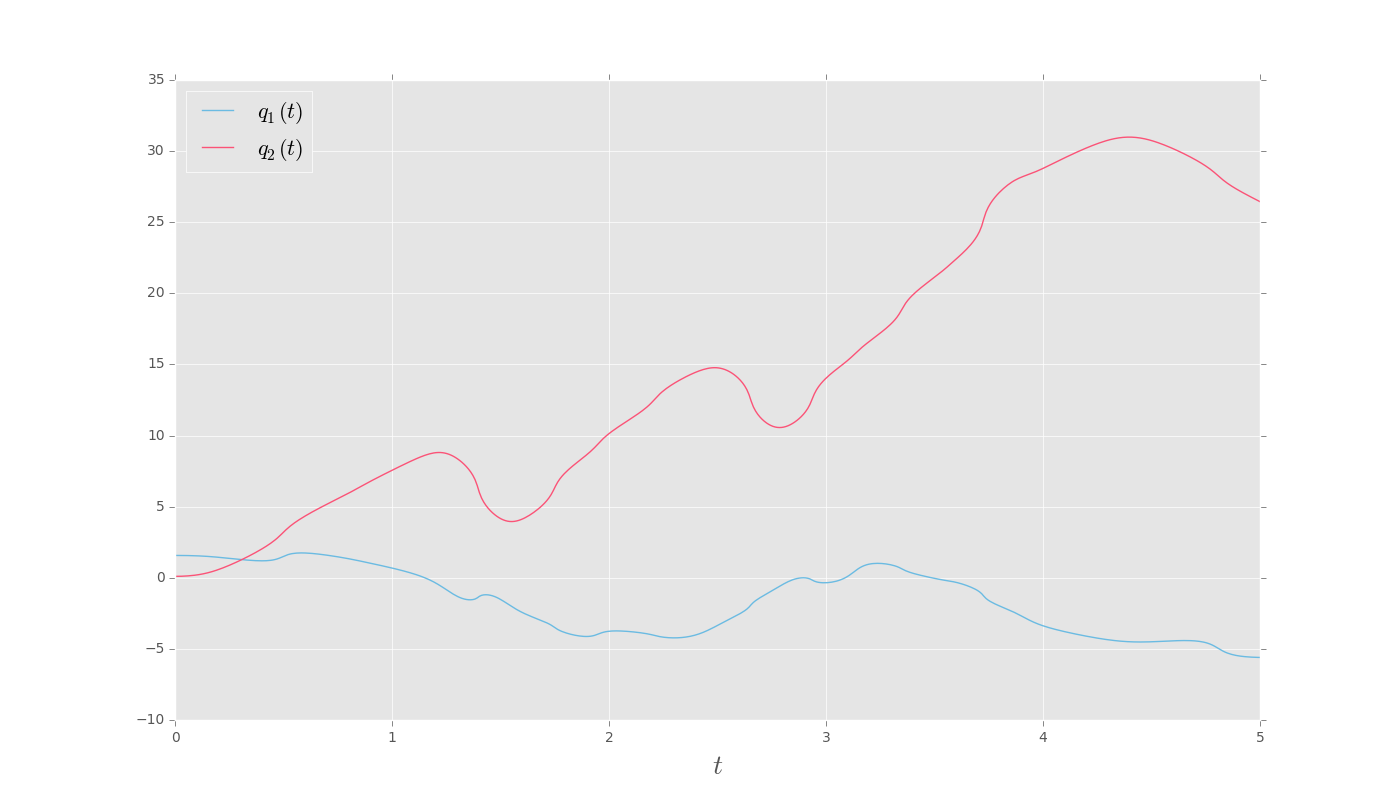
\includegraphics[width=\linewidth]{./imagenes/trayectoriaspendubotlibre.png}
\end{center}

    \begin{Verbatim}[commandchars=\\\{\}]
{\color{incolor}In [{\color{incolor}9}]:} \PY{n}{graficaxy}\PY{p}{(}\PY{l+s}{\PYZdq{}}\PY{l+s}{./imagenes/xypendubotlibre.png}\PY{l+s}{\PYZdq{}}\PY{p}{,} \PY{n}{x}\PY{p}{,} \PY{p}{[}\PY{l+s}{r\PYZsq{}}\PY{l+s}{\PYZdl{}q\PYZus{}1(t)\PYZdl{}}\PY{l+s}{\PYZsq{}}\PY{p}{,} \PY{l+s}{r\PYZsq{}}\PY{l+s}{\PYZdl{}q\PYZus{}2(t)\PYZdl{}}\PY{l+s}{\PYZsq{}}\PY{p}{]}\PY{p}{)}
\end{Verbatim}

\begin{center}
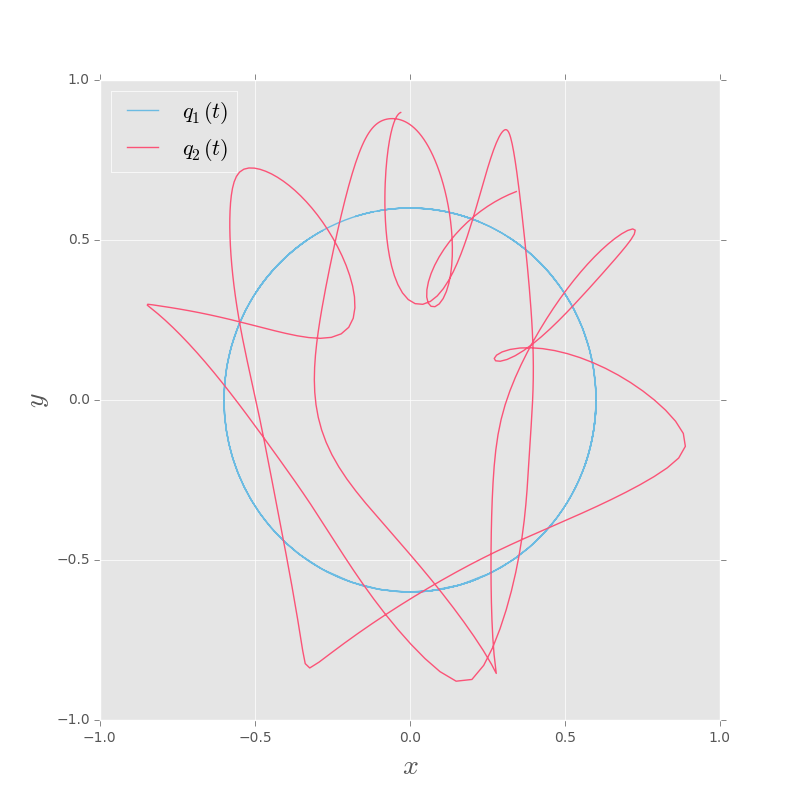
\includegraphics[width=0.5\linewidth]{./imagenes/xypendubotlibre.png}
\end{center}

    \subsection*{Linealización del modelo del
pendubot}\label{linealizaciuxf3n-del-modelo-del-pendubot}

    \subsubsection*{Estado agregado}\label{estado-agregado}

    Dado el modelo de este sistema no lineal que hemos obtenido, podemos
linealizar alrededor de los puntos de equilibrio, pero primero tenemos
que obtener las ecuaciones del sistema agregado, de tal manera que:

\[
\dot{x} = f(x, u)
\]

por lo que primero convertimos el modelo representado por una ecuación
diferencial de segundo orden, por uno representado por una ecuación
diferencial ordinaria de primer orden. Recordemos el modelo obtenido:

\[
M(q) \ddot{q} + C(q, \dot{q}) \dot{q} + U_q = G u \implies \ddot{q} = M^{-1}(q) \left[ G u - C(q, \dot{q}) \dot{q} - U_q \right]
\]

Si definimos el estado \(x\) como:

\[
x =
\begin{pmatrix}
x_1 \\
x_2 \\
x_3 \\
x_4
\end{pmatrix} =
\begin{pmatrix}
q_1 \\
q_2 \\
\dot{q}_1 \\
\dot{q}_2
\end{pmatrix}
\]

significa que tenemos que encontrar \(f(x, u)\) tal que:

\[
\dot{x} =
\begin{pmatrix}
\dot{x}_1 \\
\dot{x}_2 \\
\dot{x}_3 \\
\dot{x}_4
\end{pmatrix} =
\begin{pmatrix}
\dot{q}_1 \\
\dot{q}_2 \\
\ddot{q}_1 \\
\ddot{q}_2
\end{pmatrix} =
\begin{pmatrix}
f_1(x, u) \\
f_2(x, u) \\
f_3(x, u) \\
f_4(x, u)
\end{pmatrix} = f(x, u)
\]

en donde \(f_1\) y \(f_2\), trivialmente son:

\[
\begin{align}
f_1(x, u) &= x_3 = \dot{q}_1 \\
f_2(x, u) &= x_4 = \dot{q}_2
\end{align}
\]

y \(f_3\) y \(f_4\) estan dadas por el modelo obtenido:

\[
\begin{pmatrix}
\ddot{q}_1 \\
\ddot{q}_2
\end{pmatrix} = \ddot{q} = M^{-1}(q) \left[ G u - C(q, \dot{q}) \dot{q} - U_q \right] =
\begin{pmatrix}
f_3(x, u) \\
f_4(x, u)
\end{pmatrix}
\]

por lo que ahora debemos obtener expresiones escalares para la dinámica
del pendubot obtenida.

    \subsubsection*{Ecuaciones escalares de la dinámica del
pendubot}\label{ecuaciones-escalares-de-la-dinuxe1mica-del-pendubot}

Empezamos calculando \(M^{-1}(q)\):

\[
\begin{align}
M^{-1}(q) &= \frac{1}{\det{\left( M(q) \right)}} \adjunta{\left( M(q) \right)} \\
&= \frac{1}{\mu_1 \mu_2 - \mu_3^2 \cos^2{(q_2)}}
\begin{pmatrix}
\mu_2 & -\mu_2 - \mu_3 \cos{(q_2)} \\
-\mu_2 - \mu_3 \cos{(q_2)} & \mu_1 + \mu_2 + 2 \mu_3 \cos{(q_2)}
\end{pmatrix}
\end{align}
\]

y las ecuaciones que queremos obtener:

\[
\begin{pmatrix}
f_3(x, u) \\
f_4(x, u)
\end{pmatrix} = M^{-1}(q) G u - M^{-1}(q) C(q, \dot{q}) \dot{q} - M^{-1}(q) U_q
\]

tienen terminos:

\[
\begin{align}
M^{-1}(q) G u &= \frac{1}{\mu_1 \mu_2 - \mu_3^2 \cos^2{(q_2)}}
\begin{pmatrix}
\mu_2 & -\mu_2 - \mu_3 \cos{(q_2)} \\
-\mu_2 - \mu_3 \cos{(q_2)} & \mu_1 + \mu_2 + 2 \mu_3 \cos{(q_2)}
\end{pmatrix}
\begin{pmatrix}
1 \\
0
\end{pmatrix} u \\
&= \frac{1}{\mu_1 \mu_2 - \mu_3^2 \cos^2{(q_2)}}
\begin{pmatrix}
\mu_2 \\
-\mu_2 - \mu_3 \cos{(q_2)}
\end{pmatrix} u
\end{align}
\]

\[
\begin{align}
- M^{-1}(q) C(q, \dot{q}) \dot{q} &= \frac{\mu_3 \sin{(q_2)}}{\mu_1 \mu_2 - \mu_3^2 \cos^2{(q_2)}}
\begin{pmatrix}
\mu_2 & -\mu_2 - \mu_3 \cos{(q_2)} \\
-\mu_2 - \mu_3 \cos{(q_2)} & \mu_1 + \mu_2 + 2 \mu_3 \cos{(q_2)}
\end{pmatrix}
\begin{pmatrix}
\dot{q}_2 & \dot{q}_1 + \dot{q}_2 \\
-\dot{q}_1 & 0
\end{pmatrix} \dot{q} \\
&= \frac{\mu_3 \sin{(q_2)}}{\mu_1 \mu_2 - \mu_3^2 \cos^2{(q_2)}}
\begin{pmatrix}
\mu_2 \left( \dot{q}_1 + \dot{q}_2 \right)^2 + \mu_3 \cos{(q_2)} \dot{q}_1^2 \\
-\mu_1 \dot{q}_1^2 - \mu_2 \left( \dot{q}_1 + \dot{q}_2 \right)^2 - \mu_3 \cos{(q_2)} \left[ \left( \dot{q}_1 + \dot{q}_2 \right)^2 + \dot{q}_1^2 \right]
\end{pmatrix}
\end{align}
\]

\[
\begin{align}
-M^{-1}(q) U_q &= - \frac{g}{\mu_1 \mu_2 - \mu_3^2 \cos^2{(q_2)}}
\begin{pmatrix}
\mu_2 & -\mu_2 - \mu_3 \cos{(q_2)} \\
-\mu_2 - \mu_3 \cos{(q_2)} & \mu_1 + \mu_2 + 2 \mu_3 \cos{(q_2)}
\end{pmatrix}
\begin{pmatrix}
\mu_4 \cos{(q_1)} + \mu_5 \cos{(q_1 + q_2)} \\
\mu_5 \cos{(q_1 + q_2)}
\end{pmatrix} \\
&= - \frac{g}{\mu_1 \mu_2 - \mu_3^2 \cos^2{(q_2)}}
\begin{pmatrix}
\mu_2 \mu_4 \cos{(q_1)} - \mu_3 \mu_5 \cos{(q_2)} \cos{(q_1 + q_2)} \\
-\mu_2 \mu_4 \cos{(q_1)} - \mu_3 \mu_4 \cos{(q_1)} \cos{(q_2)} + \mu_1 \mu_5 \cos{(q_1 + q_2)} + \mu_3 \mu_5 \cos{(q_2)} \cos{(q_1 + q_2)}
\end{pmatrix}
\end{align}
\]

Por lo que al juntar todos los terminos, y hacer un poco de algebra,
tendremos que:

\[
f_3(x, u) = \frac{\mu_2 u + \mu_3 \mu_5 \sin{(q_2)} \left[ l_2 \left( \dot{q}_1 + \dot{q}_2 \right)^2 + l_1 \cos{(q_2)} \dot{q}_1^2 \right] -g \mu_3 \left[ \mu_4 \cos{(q_1)} + \mu_5 \cos{(q_2)} \cos{(q_1 + q_2)} \right]}{\mu_1 \mu_2 - \mu_3^2 \cos^2{(q_2)}}
\]

\[
\begin{align}
f_4(x, u) &= \frac{-\mu_5 \left( l_2 + l_1 \cos{(q_2)} \right)u - \mu_3 \sin{(q_2)} \left\{ m_1 l_1^2 \dot{q}_1^2 + \mu_5 \left[ \left( l_2 + l_1 \cos{(q_2)} \right) \left( \dot{q}_1 + \dot{q}_2 \right)^2 + l_1 \cos{(q_2)} \dot{q}_1^2 \right] \right\}}{\mu_1 \mu_2 - \mu_3^2 \cos^2{(q_2)}} \\
&+ \frac{g \mu_3 \left[ \left( m_1 + m_2 \right)\left( l_2 \cos{(q_1)} + l_1 \sin{(q_1)} \sin{(q_2)} \right) - \mu_5 \cos{(q_2)} \cos{(q_1 + q_2)} \right]}{\mu_1 \mu_2 - \mu_3^2 \cos^2{(q_2)}}
\end{align}
\]

    \subsubsection*{Linealización del sistema no
lineal}\label{linealizaciuxf3n-del-sistema-no-lineal}

    Dado este sistema no lineal, podemos obtener una linealización alrededor
de algun punto de equilibrio al considerar la expansión de Taylor de la
dinámica del sistema

\[
f(x, u) = f(\bar{x}, \bar{u}) + \left. \frac{\partial f}{\partial x} \right|_{x=\bar{x}, u=\bar{u}} (x - \bar{x}) + \left. \frac{\partial f}{\partial u} \right|_{x=\bar{x}, u=\bar{u}} (u - \bar{u}) + o(x, u)
\]

en donde \(f(\bar{x}, \bar{u}) = 0\) y \(o(x, u)\) son terminos de orden
superior, por lo que al tener en cuenta variaciones pequeñas de nuestra
diámica, podemos despreciarlas y obtener:

\[
\dot{\xi} = A \xi + B u
\]

en donde \(\xi = x - \bar{x}\) es el estado de nuestra linealización, y
\(A\) y \(B\) estan dados por:

\[
\begin{align}
A &= \left. \frac{\partial f}{\partial x} \right|_{x=\bar{x}, u=\bar{u}} \\
B &= \left. \frac{\partial f}{\partial u} \right|_{x=\bar{x}, u=\bar{u}}
\end{align}
\]

Calculando estas derivadas, tenemos que nuestra linealización queda:

\[
A =
\begin{pmatrix}
0 & 0 & 1 & 0 \\
0 & 0 & 0 & 1 \\
\frac{g}{l_1} & -\frac{g m_2}{l_1 m_1} & 0 & 0 \\
-\frac{g}{l_1} & \frac{g}{m_1} \left( \frac{m_1}{l_2} + \frac{m_2}{l_2} + \frac{m_2}{l_1} \right) & 0 & 0
\end{pmatrix}
\]

\[
B =
\begin{pmatrix}
0 \\
0 \\
\frac{1}{m_1 l_1^2} \\
- \frac{l_1 + l_2}{m_1 l_1^2 l_2}
\end{pmatrix}
\]

    \begin{Verbatim}[commandchars=\\\{\}]
{\color{incolor}In [{\color{incolor}12}]:} \PY{k}{def} \PY{n+nf}{f\PYZus{}lineal}\PY{p}{(}\PY{n}{x}\PY{p}{,} \PY{n}{t}\PY{p}{,} \PY{n}{K}\PY{p}{)}\PY{p}{:}
             \PY{l+s+sd}{\PYZsq{}\PYZsq{}\PYZsq{}Modelo matematico lineal pendubot}
         \PY{l+s+sd}{    Esta función f\PYZus{}lineal es tal que ẋ = f(x, t), es decir, dado el estado del sistema \PYZdq{}x\PYZdq{}}
         \PY{l+s+sd}{    y el tiempo \PYZdq{}t\PYZdq{}, devuelve la derivada en el tiempo \PYZdq{}t\PYZdq{}. Para el caso del pendubot,}
         \PY{l+s+sd}{    es invariante en el tiempo, por lo que es equivalente a ẋ = f(x).}
         
         \PY{l+s+sd}{    Ejemplo}
         \PY{l+s+sd}{    \PYZhy{}\PYZhy{}\PYZhy{}\PYZhy{}\PYZhy{}\PYZhy{}\PYZhy{}}
         \PY{l+s+sd}{    \PYZgt{}\PYZgt{}\PYZgt{} x = [τ/4, 0.1, 0, 0]}
         \PY{l+s+sd}{    \PYZgt{}\PYZgt{}\PYZgt{} t = 0}
         \PY{l+s+sd}{    \PYZgt{}\PYZgt{}\PYZgt{} f(x, t)}
         \PY{l+s+sd}{    [0.0, 0.0, \PYZhy{}4.905000000000001, 17.985]}
         \PY{l+s+sd}{    \PYZsq{}\PYZsq{}\PYZsq{}}
             
             \PY{k+kn}{from} \PY{n+nn}{numpy} \PY{k}{import} \PY{n}{matrix}\PY{p}{,} \PY{n}{zeros}\PY{p}{,} \PY{n}{cos}\PY{p}{,} \PY{n}{sin}
             
             \PY{c}{\PYZsh{} Constantes fisicas del sistema}
             \PY{n}{m1} \PY{o}{=} \PY{l+m+mf}{0.2} \PY{c}{\PYZsh{} kg}
             \PY{n}{m2} \PY{o}{=} \PY{l+m+mf}{0.6} \PY{c}{\PYZsh{} kg}
             \PY{n}{l1} \PY{o}{=} \PY{l+m+mf}{0.6} \PY{c}{\PYZsh{} m}
             \PY{n}{l2} \PY{o}{=} \PY{l+m+mf}{0.3} \PY{c}{\PYZsh{} m}
             \PY{n}{g} \PY{o}{=} \PY{l+m+mf}{9.81} \PY{c}{\PYZsh{} m/s\PYZca{}2}
             
             \PY{c}{\PYZsh{} Matriz sistema linealizado}
             \PY{n}{A} \PY{o}{=} \PY{n}{matrix}\PY{p}{(}\PY{p}{[}\PY{p}{[}\PY{l+m+mi}{0}\PY{p}{,} \PY{l+m+mi}{0}\PY{p}{,} \PY{l+m+mi}{1}\PY{p}{,} \PY{l+m+mi}{0}\PY{p}{]}\PY{p}{,}
                         \PY{p}{[}\PY{l+m+mi}{0}\PY{p}{,} \PY{l+m+mi}{0}\PY{p}{,} \PY{l+m+mi}{0}\PY{p}{,} \PY{l+m+mi}{1}\PY{p}{]}\PY{p}{,}
                         \PY{p}{[}\PY{n}{g}\PY{o}{/}\PY{n}{l1}\PY{p}{,} \PY{o}{\PYZhy{}}\PY{n}{g}\PY{o}{*}\PY{n}{m2}\PY{o}{/}\PY{p}{(}\PY{n}{l1}\PY{o}{*}\PY{n}{m1}\PY{p}{)}\PY{p}{,} \PY{l+m+mi}{0}\PY{p}{,} \PY{l+m+mi}{0}\PY{p}{]}\PY{p}{,}
                         \PY{p}{[}\PY{o}{\PYZhy{}}\PY{n}{g}\PY{o}{/}\PY{n}{l1}\PY{p}{,} \PY{n}{g}\PY{o}{/}\PY{n}{m1}\PY{o}{*}\PY{p}{(}\PY{n}{m1}\PY{o}{/}\PY{n}{l2} \PY{o}{+} \PY{n}{m2}\PY{o}{/}\PY{n}{l2} \PY{o}{+} \PY{n}{m2}\PY{o}{/}\PY{n}{l1}\PY{p}{)}\PY{p}{,} \PY{l+m+mi}{0}\PY{p}{,} \PY{l+m+mi}{0}\PY{p}{]}\PY{p}{]}\PY{p}{)}
             
             \PY{c}{\PYZsh{} Vector de entrada}
             \PY{n}{B} \PY{o}{=} \PY{n}{matrix}\PY{p}{(}\PY{p}{[}\PY{p}{[}\PY{l+m+mi}{0}\PY{p}{]}\PY{p}{,}\PY{p}{[}\PY{l+m+mi}{0}\PY{p}{]}\PY{p}{,}\PY{p}{[}\PY{l+m+mi}{1}\PY{o}{/}\PY{p}{(}\PY{n}{m1}\PY{o}{*}\PY{n}{l1}\PY{o}{*}\PY{o}{*}\PY{l+m+mi}{2}\PY{p}{)}\PY{p}{]}\PY{p}{,}\PY{p}{[}\PY{o}{\PYZhy{}}\PY{p}{(}\PY{n}{l1} \PY{o}{+} \PY{n}{l2}\PY{p}{)}\PY{o}{/}\PY{p}{(}\PY{n}{m1}\PY{o}{*}\PY{n}{l1}\PY{o}{*}\PY{o}{*}\PY{l+m+mi}{2}\PY{o}{*}\PY{n}{l2}\PY{p}{)}\PY{p}{]}\PY{p}{]}\PY{p}{)}
             
             \PY{c}{\PYZsh{} Ley de control lineal}
             \PY{n}{u} \PY{o}{=} \PY{o}{\PYZhy{}}\PY{n}{matrix}\PY{p}{(}\PY{n}{K}\PY{p}{)}\PY{o}{*}\PY{n}{matrix}\PY{p}{(}\PY{n}{x}\PY{p}{)}\PY{o}{.}\PY{n}{T}
             
             \PY{c}{\PYZsh{} Dinámica del sistema linealizado}
             \PY{n}{ẋ} \PY{o}{=} \PY{n}{A}\PY{o}{*}\PY{n}{matrix}\PY{p}{(}\PY{n}{x}\PY{p}{)}\PY{o}{.}\PY{n}{T} \PY{o}{+} \PY{n}{B}\PY{o}{*}\PY{n}{u}
             
             \PY{c}{\PYZsh{} Se devuelve la derivada}
             \PY{k}{return} \PY{p}{(}\PY{n}{ẋ}\PY{o}{.}\PY{n}{T}\PY{p}{)}\PY{o}{.}\PY{n}{tolist}\PY{p}{(}\PY{p}{)}\PY{p}{[}\PY{l+m+mi}{0}\PY{p}{]}
\end{Verbatim}

    \begin{Verbatim}[commandchars=\\\{\}]
{\color{incolor}In [{\color{incolor}13}]:} \PY{n}{ts} \PY{o}{=} \PY{n}{linspace}\PY{p}{(}\PY{l+m+mi}{0}\PY{p}{,} \PY{l+m+mf}{0.4}\PY{p}{,} \PY{l+m+mi}{100}\PY{p}{)}
         \PY{n}{estado\PYZus{}inicial\PYZus{}lineal} \PY{o}{=} \PY{p}{[}\PY{l+m+mf}{0.0}\PY{p}{,} \PY{l+m+mf}{0.1}\PY{p}{,} \PY{l+m+mf}{0.0}\PY{p}{,} \PY{l+m+mf}{0.0}\PY{p}{]}
         
         \PY{n}{f\PYZus{}lineal\PYZus{}libre} \PY{o}{=} \PY{k}{lambda} \PY{n}{x}\PY{p}{,} \PY{n}{t}\PY{p}{:} \PY{n}{f\PYZus{}lineal}\PY{p}{(}\PY{n}{x}\PY{p}{,} \PY{n}{t}\PY{p}{,} \PY{p}{[}\PY{l+m+mi}{0}\PY{p}{,} \PY{l+m+mi}{0}\PY{p}{,} \PY{l+m+mi}{0}\PY{p}{,} \PY{l+m+mi}{0}\PY{p}{]}\PY{p}{)}
         
         \PY{n}{ξs} \PY{o}{=} \PY{n}{odeint}\PY{p}{(}\PY{n}{f\PYZus{}lineal\PYZus{}libre}\PY{p}{,} \PY{n}{estado\PYZus{}inicial\PYZus{}lineal}\PY{p}{,} \PY{n}{ts}\PY{p}{)}
         \PY{n}{xl} \PY{o}{=} \PY{n}{array}\PY{p}{(}\PY{p}{[}\PY{n}{ξ} \PY{o}{+} \PY{n}{array}\PY{p}{(}\PY{p}{[}\PY{n}{τ}\PY{o}{/}\PY{l+m+mi}{4}\PY{p}{,} \PY{l+m+mi}{0}\PY{p}{,} \PY{l+m+mi}{0}\PY{p}{,} \PY{l+m+mi}{0}\PY{p}{]}\PY{p}{)} \PY{k}{for} \PY{n}{ξ} \PY{o+ow}{in} \PY{n}{ξs}\PY{p}{]}\PY{p}{)}
\end{Verbatim}

    \begin{Verbatim}[commandchars=\\\{\}]
{\color{incolor}In [{\color{incolor}14}]:} \PY{n}{graficatemporal}\PY{p}{(}\PY{l+s}{\PYZdq{}}\PY{l+s}{./imagenes/trayectoriaspendubotlineallibre.png}\PY{l+s}{\PYZdq{}}\PY{p}{,} \PY{n}{xl}\PY{p}{,} \PY{n}{ts}\PY{p}{,} \PY{p}{[}\PY{l+s}{r\PYZsq{}}\PY{l+s}{\PYZdl{}}\PY{l+s}{\PYZbs{}}\PY{l+s}{xi\PYZus{}1(t) + }\PY{l+s}{\PYZbs{}}\PY{l+s}{frac\PYZob{}}\PY{l+s}{\PYZbs{}}\PY{l+s}{tau\PYZcb{}\PYZob{}4\PYZcb{}\PYZdl{}}\PY{l+s}{\PYZsq{}}\PY{p}{,} \PY{l+s}{r\PYZsq{}}\PY{l+s}{\PYZdl{}}\PY{l+s}{\PYZbs{}}\PY{l+s}{xi\PYZus{}2(t)\PYZdl{}}\PY{l+s}{\PYZsq{}}\PY{p}{]}\PY{p}{)}
\end{Verbatim}

\begin{center}
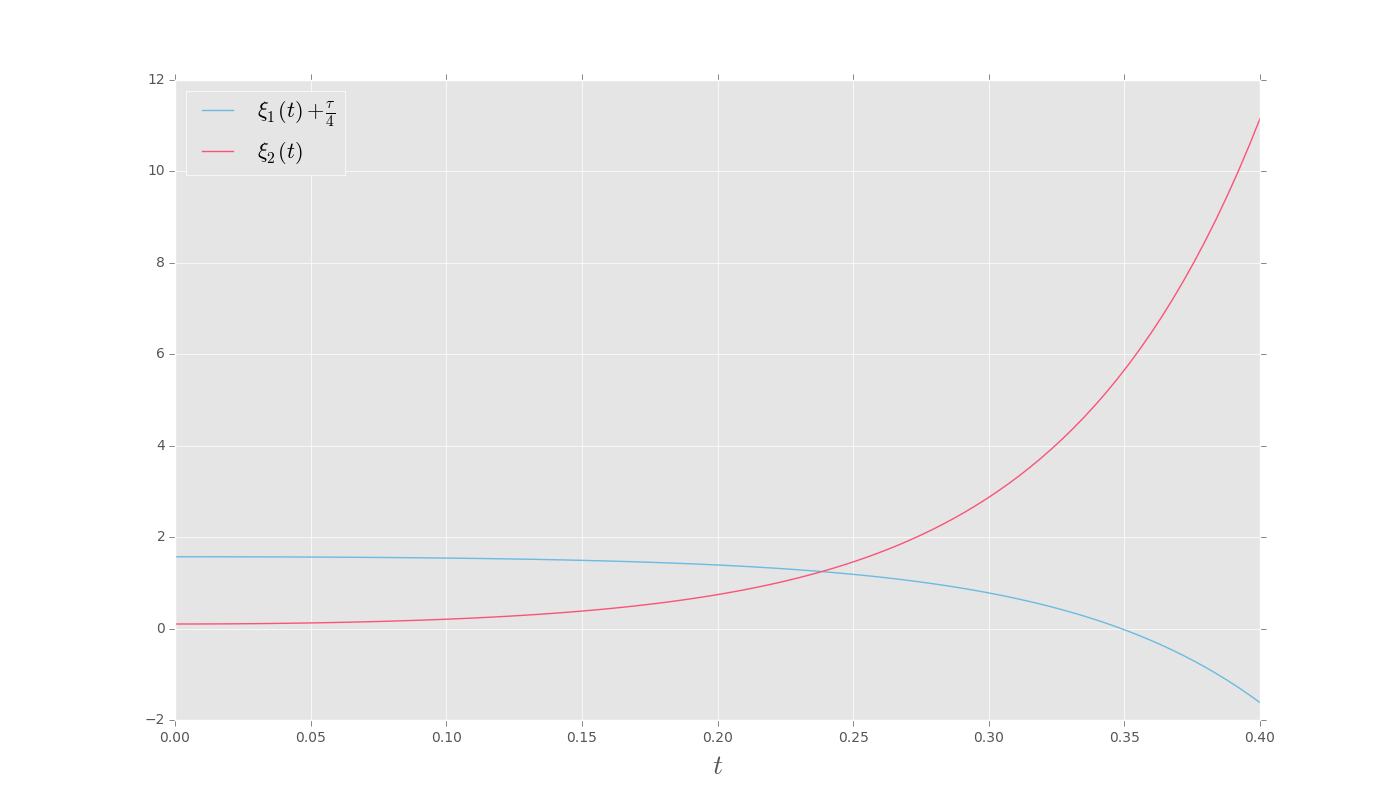
\includegraphics[width=\linewidth]{./imagenes/trayectoriaspendubotlineallibre.png}
\end{center}

    \begin{Verbatim}[commandchars=\\\{\}]
{\color{incolor}In [{\color{incolor}15}]:} \PY{n}{graficaxy}\PY{p}{(}\PY{l+s}{\PYZdq{}}\PY{l+s}{./imagenes/xypendubotlineallibre.png}\PY{l+s}{\PYZdq{}}\PY{p}{,} \PY{n}{xl}\PY{p}{,} \PY{p}{[}\PY{l+s}{r\PYZsq{}}\PY{l+s}{\PYZdl{}}\PY{l+s}{\PYZbs{}}\PY{l+s}{xi\PYZus{}1(t) + }\PY{l+s}{\PYZbs{}}\PY{l+s}{frac\PYZob{}}\PY{l+s}{\PYZbs{}}\PY{l+s}{tau\PYZcb{}\PYZob{}4\PYZcb{}\PYZdl{}}\PY{l+s}{\PYZsq{}}\PY{p}{,} \PY{l+s}{r\PYZsq{}}\PY{l+s}{\PYZdl{}}\PY{l+s}{\PYZbs{}}\PY{l+s}{xi\PYZus{}2(t)\PYZdl{}}\PY{l+s}{\PYZsq{}}\PY{p}{]}\PY{p}{)}
\end{Verbatim}

\begin{center}
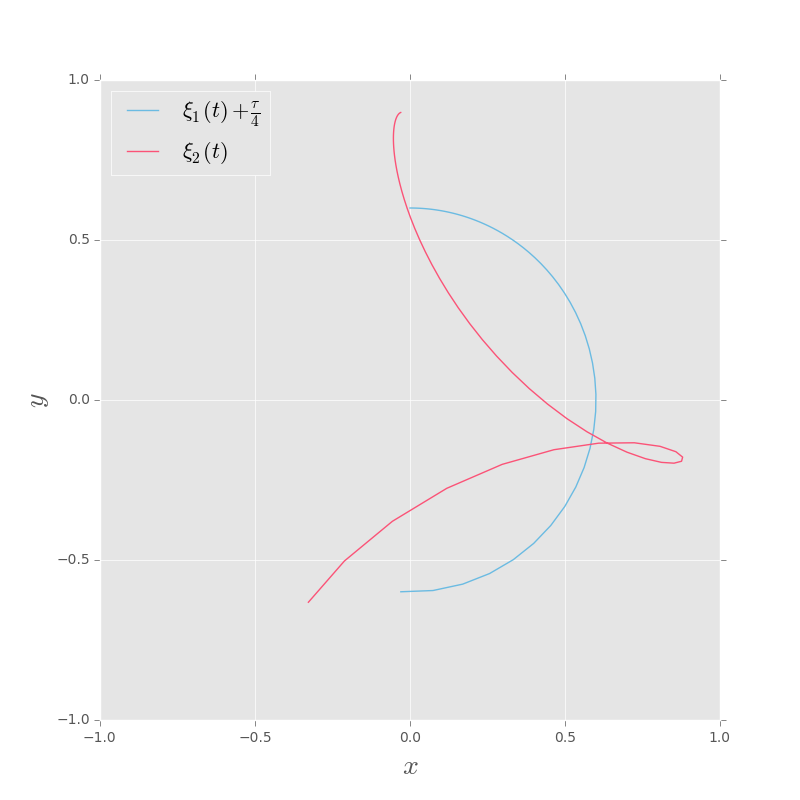
\includegraphics[width=0.5\linewidth]{./imagenes/xypendubotlineallibre.png}
\end{center}

\begin{center}
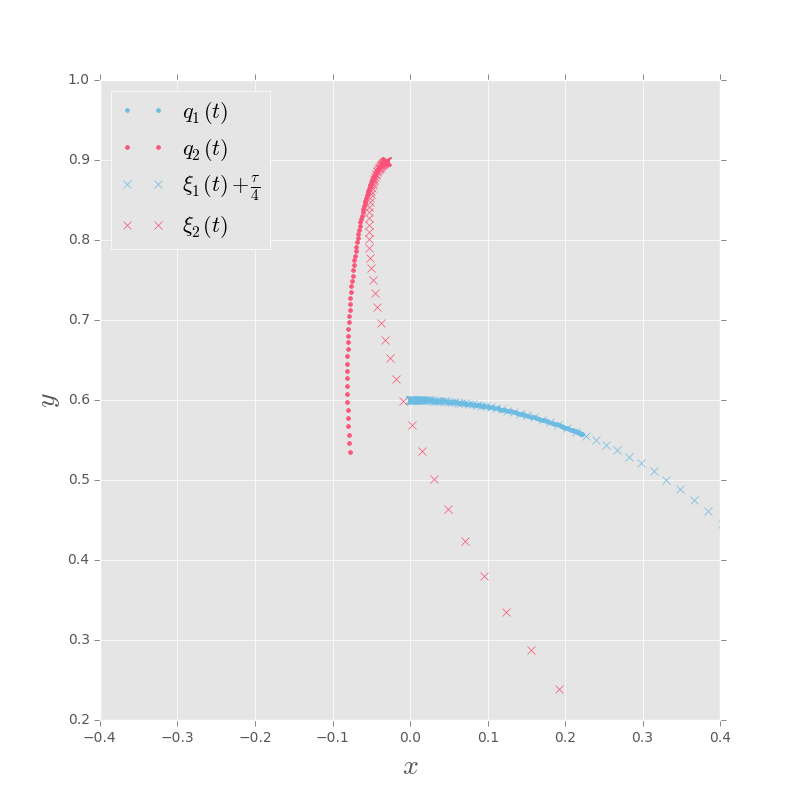
\includegraphics[width=0.5\linewidth]{./imagenes/xypendubotlinealynolineallibres.png}
\end{center}

    Aqui podemos ver como el sistema linealizado deverge rapidamente del
sistema original, por lo que podemos asumer que este modelo linealizado
es valido para variaciones muy pequeñas de \(q_1\) y \(q_2\).

    \subsection*{Diseño de un control
óptimo}\label{diseuxf1o-de-un-control-uxf3ptimo}

    Para el diseño de la ley de control óptima que minimice la funcional:

\[
J(u) = \int_0^{\infty} \left( x^T(t) Q x(t) + u^2(t) \right) dt
\]

con \(Q\) de la forma:

\[
Q =
\begin{pmatrix}
1 & 0 & 0 & 0 \\
0 & 1 & 0 & 0 \\
0 & 0 & 10 & 0 \\
0 & 0 & 0 & 10
\end{pmatrix}
\]

tal que la ley de control óptima sea:

\[
u^*(t) = -K \xi^*(t)
\]

Para calcular la ganancia \(K\) asociada a esta función de costo,
utilizaremos el sistema lineal encontrado.

    \begin{Verbatim}[commandchars=\\\{\}]
{\color{incolor}In [{\color{incolor}18}]:} \PY{k+kn}{from} \PY{n+nn}{control} \PY{k}{import} \PY{n}{lqr}
         \PY{k+kn}{from} \PY{n+nn}{numpy} \PY{k}{import} \PY{n}{matrix}
\end{Verbatim}

    \begin{Verbatim}[commandchars=\\\{\}]
{\color{incolor}In [{\color{incolor}19}]:} \PY{n}{m1} \PY{o}{=} \PY{l+m+mf}{0.2} \PY{c}{\PYZsh{} kg}
         \PY{n}{m2} \PY{o}{=} \PY{l+m+mf}{0.6} \PY{c}{\PYZsh{} kg}
         \PY{n}{l1} \PY{o}{=} \PY{l+m+mf}{0.6} \PY{c}{\PYZsh{} m}
         \PY{n}{l2} \PY{o}{=} \PY{l+m+mf}{0.3} \PY{c}{\PYZsh{} m}
         \PY{n}{g} \PY{o}{=} \PY{l+m+mf}{9.81} \PY{c}{\PYZsh{} m/s\PYZca{}2}
         
         \PY{n}{A} \PY{o}{=} \PY{n}{matrix}\PY{p}{(}\PY{p}{[}\PY{p}{[}\PY{l+m+mi}{0}\PY{p}{,} \PY{l+m+mi}{0}\PY{p}{,} \PY{l+m+mi}{1}\PY{p}{,} \PY{l+m+mi}{0}\PY{p}{]}\PY{p}{,}
                     \PY{p}{[}\PY{l+m+mi}{0}\PY{p}{,} \PY{l+m+mi}{0}\PY{p}{,} \PY{l+m+mi}{0}\PY{p}{,} \PY{l+m+mi}{1}\PY{p}{]}\PY{p}{,}
                     \PY{p}{[}\PY{n}{g}\PY{o}{/}\PY{n}{l1}\PY{p}{,} \PY{o}{\PYZhy{}}\PY{n}{g}\PY{o}{*}\PY{n}{m2}\PY{o}{/}\PY{p}{(}\PY{n}{l1}\PY{o}{*}\PY{n}{m1}\PY{p}{)}\PY{p}{,} \PY{l+m+mi}{0}\PY{p}{,} \PY{l+m+mi}{0}\PY{p}{]}\PY{p}{,}
                     \PY{p}{[}\PY{o}{\PYZhy{}}\PY{n}{g}\PY{o}{/}\PY{n}{l1}\PY{p}{,} \PY{n}{g}\PY{o}{/}\PY{n}{m1}\PY{o}{*}\PY{p}{(}\PY{n}{m1}\PY{o}{/}\PY{n}{l2} \PY{o}{+} \PY{n}{m2}\PY{o}{/}\PY{n}{l2} \PY{o}{+} \PY{n}{m2}\PY{o}{/}\PY{n}{l1}\PY{p}{)}\PY{p}{,} \PY{l+m+mi}{0}\PY{p}{,} \PY{l+m+mi}{0}\PY{p}{]}\PY{p}{]}\PY{p}{)}
         
         \PY{n}{B} \PY{o}{=} \PY{n}{matrix}\PY{p}{(}\PY{p}{[}\PY{p}{[}\PY{l+m+mi}{0}\PY{p}{]}\PY{p}{,}
                     \PY{p}{[}\PY{l+m+mi}{0}\PY{p}{]}\PY{p}{,}
                     \PY{p}{[}\PY{l+m+mi}{1}\PY{o}{/}\PY{p}{(}\PY{n}{m1}\PY{o}{*}\PY{n}{l1}\PY{o}{*}\PY{o}{*}\PY{l+m+mi}{2}\PY{p}{)}\PY{p}{]}\PY{p}{,}
                     \PY{p}{[}\PY{o}{\PYZhy{}}\PY{p}{(}\PY{n}{l1}\PY{o}{+}\PY{n}{l2}\PY{p}{)}\PY{o}{/}\PY{p}{(}\PY{n}{m1}\PY{o}{*}\PY{n}{l1}\PY{o}{*}\PY{o}{*}\PY{l+m+mi}{2}\PY{o}{*}\PY{n}{l2}\PY{p}{)}\PY{p}{]}\PY{p}{]}\PY{p}{)}
         
         \PY{n}{Q} \PY{o}{=} \PY{n}{matrix}\PY{p}{(}\PY{p}{[}\PY{p}{[}\PY{l+m+mi}{1}\PY{p}{,} \PY{l+m+mi}{0}\PY{p}{,} \PY{l+m+mi}{0}\PY{p}{,} \PY{l+m+mi}{0}\PY{p}{]}\PY{p}{,}
                     \PY{p}{[}\PY{l+m+mi}{0}\PY{p}{,} \PY{l+m+mi}{1}\PY{p}{,} \PY{l+m+mi}{0}\PY{p}{,} \PY{l+m+mi}{0}\PY{p}{]}\PY{p}{,}
                     \PY{p}{[}\PY{l+m+mi}{0}\PY{p}{,} \PY{l+m+mi}{0}\PY{p}{,} \PY{l+m+mi}{10}\PY{p}{,} \PY{l+m+mi}{0}\PY{p}{]}\PY{p}{,}
                     \PY{p}{[}\PY{l+m+mi}{0}\PY{p}{,} \PY{l+m+mi}{0}\PY{p}{,} \PY{l+m+mi}{0}\PY{p}{,} \PY{l+m+mi}{10}\PY{p}{]}\PY{p}{]}\PY{p}{)}
         
         \PY{n}{R} \PY{o}{=} \PY{n}{matrix}\PY{p}{(}\PY{p}{[}\PY{p}{[}\PY{l+m+mi}{1}\PY{p}{]}\PY{p}{]}\PY{p}{)}
\end{Verbatim}

    \begin{Verbatim}[commandchars=\\\{\}]
{\color{incolor}In [{\color{incolor}20}]:} \PY{n}{K}\PY{p}{,} \PY{n}{S}\PY{p}{,} \PY{n}{E} \PY{o}{=} \PY{n}{lqr}\PY{p}{(}\PY{n}{A}\PY{p}{,} \PY{n}{B}\PY{p}{,} \PY{n}{Q}\PY{p}{,} \PY{n}{R}\PY{p}{)}
         \PY{n}{K}
\end{Verbatim}

            \begin{Verbatim}[commandchars=\\\{\}]
{\color{outcolor}Out[{\color{outcolor}20}]:} array([[-51.600978  , -51.39319408, -16.05940057,  -8.92417942]])
\end{Verbatim}
        
    Una vez que hemos obtenido las ganancias de realimentacion, tan solo
tenemos que incluirlas en la simulación del sistema para ver su
desempeño.

    \begin{Verbatim}[commandchars=\\\{\}]
{\color{incolor}In [{\color{incolor}21}]:} \PY{n}{ts} \PY{o}{=} \PY{n}{linspace}\PY{p}{(}\PY{l+m+mi}{0}\PY{p}{,} \PY{l+m+mi}{5}\PY{p}{,} \PY{l+m+mi}{500}\PY{p}{)}
         \PY{n}{estado\PYZus{}inicial\PYZus{}lineal} \PY{o}{=} \PY{p}{[}\PY{l+m+mf}{0.0}\PY{p}{,} \PY{l+m+mf}{0.1}\PY{p}{,} \PY{l+m+mf}{0.0}\PY{p}{,} \PY{l+m+mf}{0.0}\PY{p}{]}
         
         \PY{n}{f\PYZus{}lineal\PYZus{}optima} \PY{o}{=} \PY{k}{lambda} \PY{n}{x}\PY{p}{,} \PY{n}{t}\PY{p}{:} \PY{n}{f\PYZus{}lineal}\PY{p}{(}\PY{n}{x}\PY{p}{,} \PY{n}{t}\PY{p}{,} \PY{n}{K}\PY{p}{)}
         
         \PY{n}{ξs} \PY{o}{=} \PY{n}{odeint}\PY{p}{(}\PY{n}{f\PYZus{}lineal\PYZus{}optima}\PY{p}{,} \PY{n}{estado\PYZus{}inicial\PYZus{}lineal}\PY{p}{,} \PY{n}{ts}\PY{p}{)}
         \PY{n}{xl} \PY{o}{=} \PY{n}{array}\PY{p}{(}\PY{p}{[}\PY{n}{ξ} \PY{o}{+} \PY{n}{array}\PY{p}{(}\PY{p}{[}\PY{n}{τ}\PY{o}{/}\PY{l+m+mi}{4}\PY{p}{,} \PY{l+m+mi}{0}\PY{p}{,} \PY{l+m+mi}{0}\PY{p}{,} \PY{l+m+mi}{0}\PY{p}{]}\PY{p}{)} \PY{k}{for} \PY{n}{ξ} \PY{o+ow}{in} \PY{n}{ξs}\PY{p}{]}\PY{p}{)}
\end{Verbatim}

    \begin{Verbatim}[commandchars=\\\{\}]
{\color{incolor}In [{\color{incolor}22}]:} \PY{n}{graficatemporal}\PY{p}{(}\PY{l+s}{\PYZdq{}}\PY{l+s}{./imagenes/trayectoriaspendubotlinealoptimo.png}\PY{l+s}{\PYZdq{}}\PY{p}{,} \PY{n}{xl}\PY{p}{,} \PY{n}{ts}\PY{p}{,} \PY{p}{[}\PY{l+s}{r\PYZsq{}}\PY{l+s}{\PYZdl{}}\PY{l+s}{\PYZbs{}}\PY{l+s}{xi\PYZus{}1(t) + }\PY{l+s}{\PYZbs{}}\PY{l+s}{frac\PYZob{}}\PY{l+s}{\PYZbs{}}\PY{l+s}{tau\PYZcb{}\PYZob{}4\PYZcb{}\PYZdl{}}\PY{l+s}{\PYZsq{}}\PY{p}{,} \PY{l+s}{r\PYZsq{}}\PY{l+s}{\PYZdl{}}\PY{l+s}{\PYZbs{}}\PY{l+s}{xi\PYZus{}2(t)\PYZdl{}}\PY{l+s}{\PYZsq{}}\PY{p}{]}\PY{p}{)}
\end{Verbatim}

\begin{center}
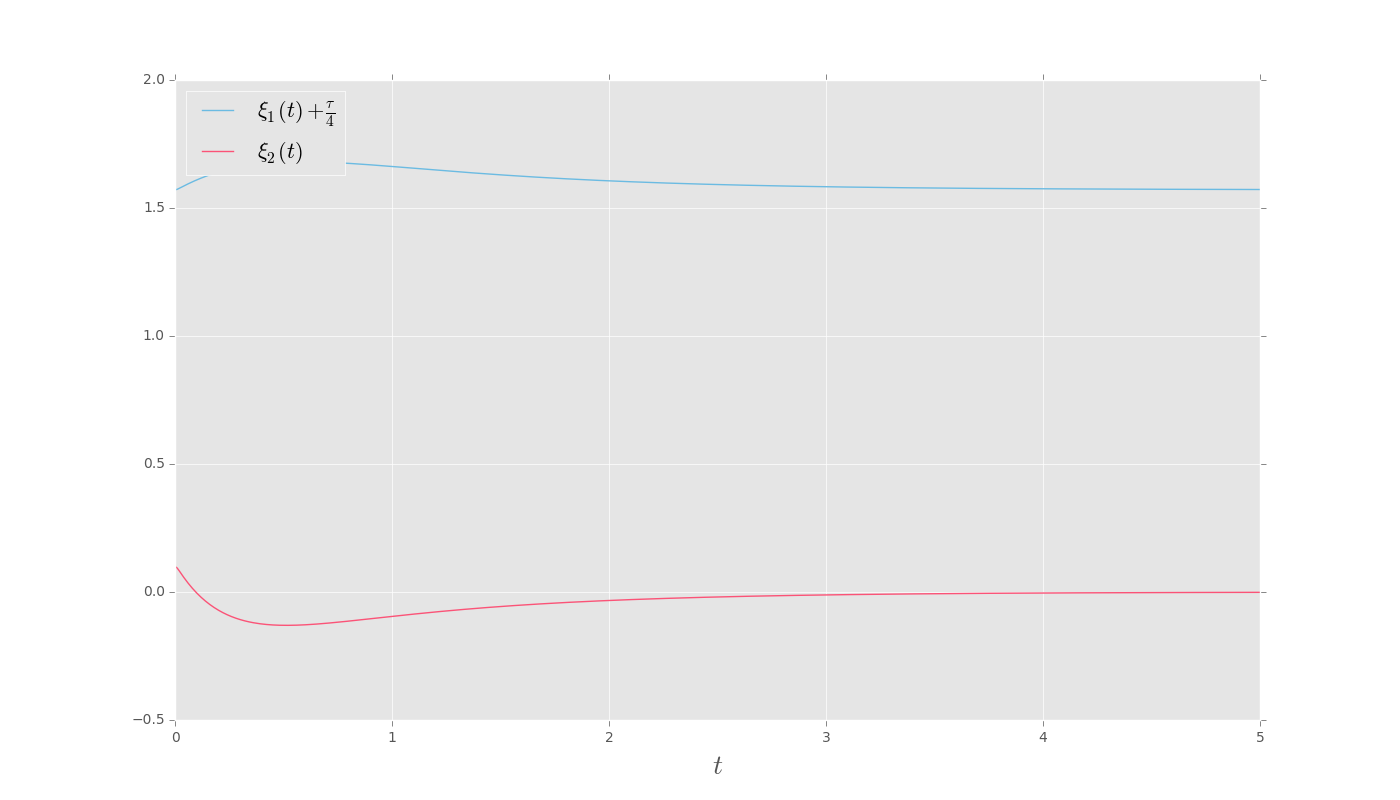
\includegraphics[width=\linewidth]{./imagenes/trayectoriaspendubotlinealoptimo.png}
\end{center}

    \begin{Verbatim}[commandchars=\\\{\}]
{\color{incolor}In [{\color{incolor}23}]:} \PY{n}{graficaxy}\PY{p}{(}\PY{l+s}{\PYZdq{}}\PY{l+s}{./imagenes/xypendubotlinealoptimo.png}\PY{l+s}{\PYZdq{}}\PY{p}{,} \PY{n}{xl}\PY{p}{,} \PY{p}{[}\PY{l+s}{r\PYZsq{}}\PY{l+s}{\PYZdl{}}\PY{l+s}{\PYZbs{}}\PY{l+s}{xi\PYZus{}1(t) + }\PY{l+s}{\PYZbs{}}\PY{l+s}{frac\PYZob{}}\PY{l+s}{\PYZbs{}}\PY{l+s}{tau\PYZcb{}\PYZob{}4\PYZcb{}\PYZdl{}}\PY{l+s}{\PYZsq{}}\PY{p}{,} \PY{l+s}{r\PYZsq{}}\PY{l+s}{\PYZdl{}}\PY{l+s}{\PYZbs{}}\PY{l+s}{xi\PYZus{}2(t)\PYZdl{}}\PY{l+s}{\PYZsq{}}\PY{p}{]}\PY{p}{)}
\end{Verbatim}

\begin{center}
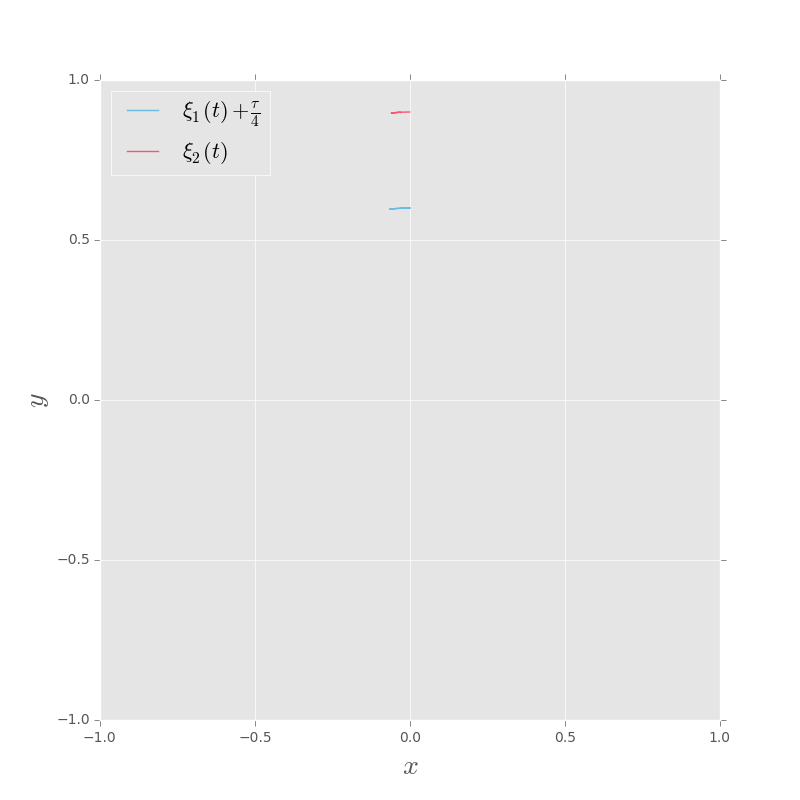
\includegraphics[width=0.5\linewidth]{./imagenes/xypendubotlinealoptimo.png}
\end{center}

    Ahora sabemos que este control estabiliza al sistema linealizado, pero
en realidad queremos saber como se desempeña con el sistema no lineal.

Podemos realimentar el sistema original para ver su desempeño.

    \begin{Verbatim}[commandchars=\\\{\}]
{\color{incolor}In [{\color{incolor}24}]:} \PY{n}{ts} \PY{o}{=} \PY{n}{linspace}\PY{p}{(}\PY{l+m+mi}{0}\PY{p}{,} \PY{l+m+mi}{5}\PY{p}{,} \PY{l+m+mi}{500}\PY{p}{)}
         \PY{n}{estado\PYZus{}inicial} \PY{o}{=} \PY{p}{[}\PY{n}{τ}\PY{o}{/}\PY{l+m+mi}{4}\PY{p}{,} \PY{l+m+mf}{0.1}\PY{p}{,} \PY{l+m+mi}{0}\PY{p}{,} \PY{l+m+mi}{0}\PY{p}{]}
         
         \PY{n}{f\PYZus{}optima} \PY{o}{=} \PY{k}{lambda} \PY{n}{x}\PY{p}{,} \PY{n}{t}\PY{p}{:} \PY{n}{f}\PY{p}{(}\PY{n}{x}\PY{p}{,} \PY{n}{t}\PY{p}{,} \PY{n}{K}\PY{p}{)}
         
         \PY{n}{x} \PY{o}{=} \PY{n}{odeint}\PY{p}{(}\PY{n}{f\PYZus{}optima}\PY{p}{,} \PY{n}{estado\PYZus{}inicial}\PY{p}{,} \PY{n}{ts}\PY{p}{)}
\end{Verbatim}

    \begin{Verbatim}[commandchars=\\\{\}]
{\color{incolor}In [{\color{incolor}25}]:} \PY{n}{graficatemporal}\PY{p}{(}\PY{l+s}{\PYZdq{}}\PY{l+s}{./imagenes/trayectoriaspendubotoptimo.png}\PY{l+s}{\PYZdq{}}\PY{p}{,} \PY{n}{x}\PY{p}{,} \PY{n}{ts}\PY{p}{,} \PY{p}{[}\PY{l+s}{r\PYZsq{}}\PY{l+s}{\PYZdl{}q\PYZus{}1(t)\PYZdl{}}\PY{l+s}{\PYZsq{}}\PY{p}{,} \PY{l+s}{r\PYZsq{}}\PY{l+s}{\PYZdl{}q\PYZus{}2(t)\PYZdl{}}\PY{l+s}{\PYZsq{}}\PY{p}{]}\PY{p}{)}
\end{Verbatim}

\begin{center}
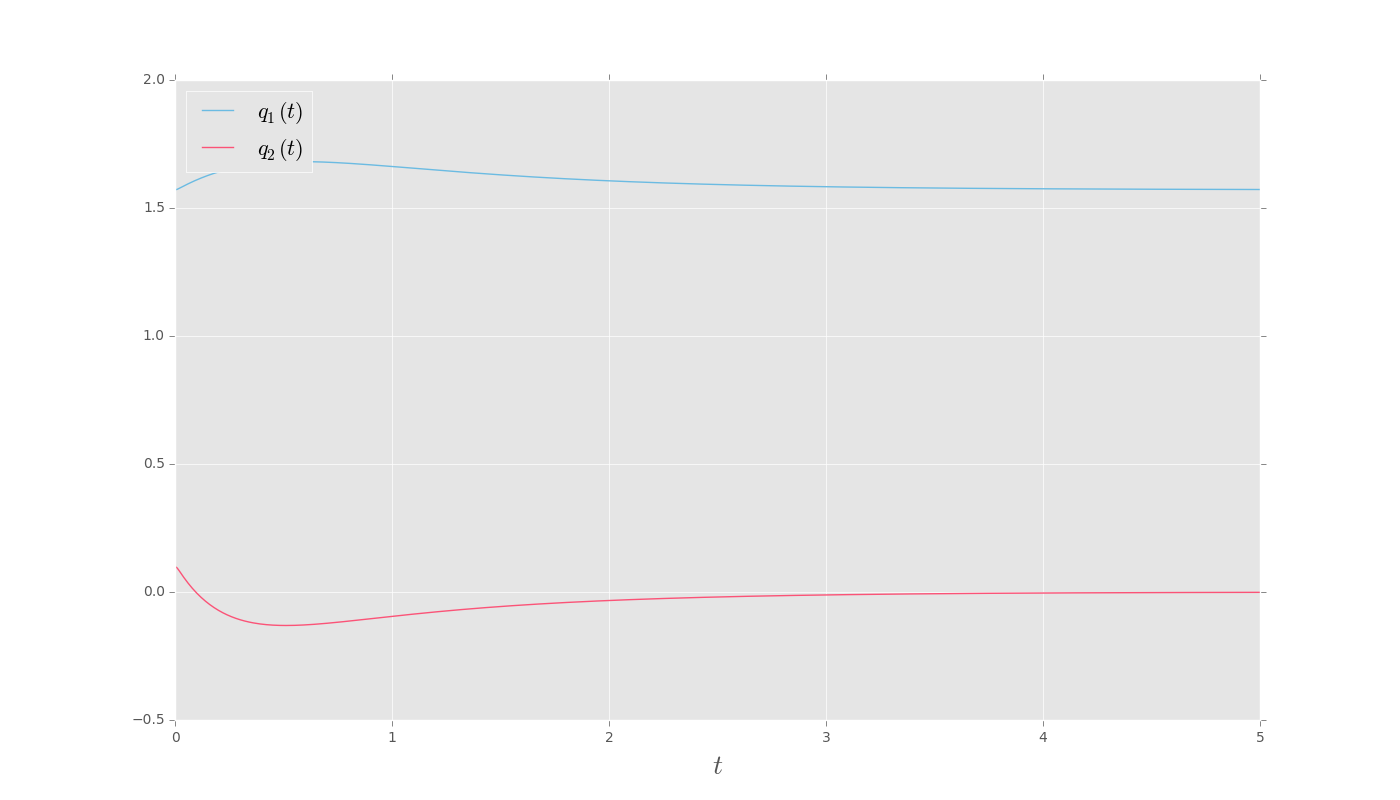
\includegraphics[width=0.9\linewidth]{./imagenes/trayectoriaspendubotoptimo.png}
\end{center}
        
    \begin{Verbatim}[commandchars=\\\{\}]
{\color{incolor}In [{\color{incolor}26}]:} \PY{n}{graficaxy}\PY{p}{(}\PY{l+s}{\PYZdq{}}\PY{l+s}{./imagenes/xypendubotoptimo.png}\PY{l+s}{\PYZdq{}}\PY{p}{,} \PY{n}{x}\PY{p}{,} \PY{p}{[}\PY{l+s}{r\PYZsq{}}\PY{l+s}{\PYZdl{}q\PYZus{}1(t)\PYZdl{}}\PY{l+s}{\PYZsq{}}\PY{p}{,} \PY{l+s}{r\PYZsq{}}\PY{l+s}{\PYZdl{}q\PYZus{}2(t)\PYZdl{}}\PY{l+s}{\PYZsq{}}\PY{p}{]}\PY{p}{)}
\end{Verbatim}

\begin{center}
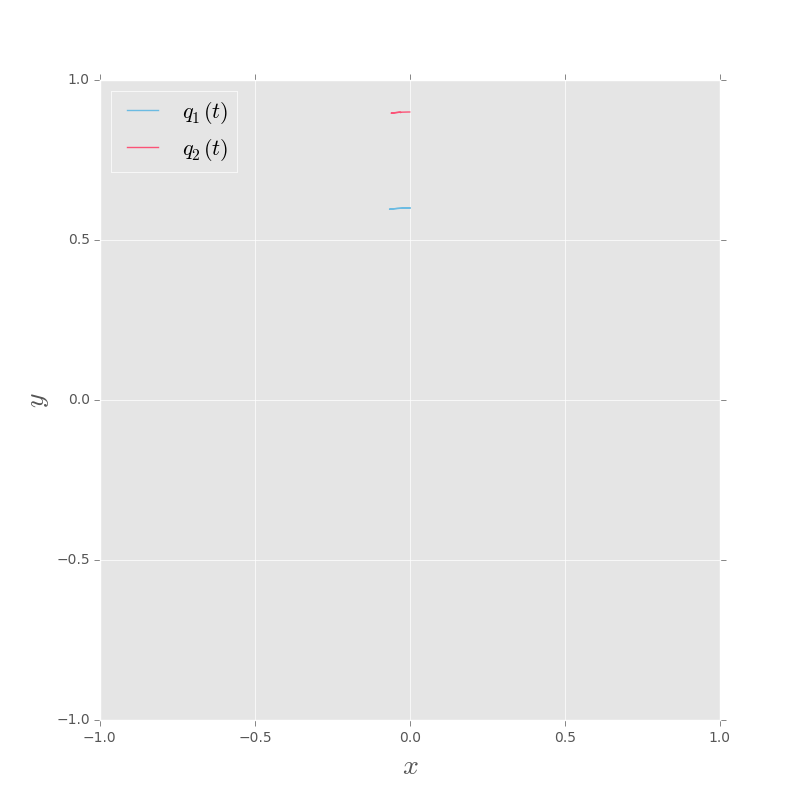
\includegraphics[width=0.5\linewidth]{./imagenes/xypendubotoptimo.png}
\end{center}
        
    Si deseas compartir este Notebook de IPython, o ver las animaciones y el codigo completo, utiliza la siguiente
dirección: http://bit.ly/1H1bR6Q, o bien el siguiente código QR:

\begin{center}

\includegraphics[width=0.2\linewidth]{codigos/pendubot.jpg}
\end{center}


    % Add a bibliography block to the postdoc
    
    
    
    \end{document}
